\chapter{Datenspeicherung}
\label{ch:data_persistence}

\section{Allgemeiner forensischer Analyseprozess}
Im Praxisteil dieser Arbeit soll eine Analyseplattform auf Basis von Apache Hadoop aufgebaut werden. Diese Analyseplattform dient zur Auswertung sichergestellter Beweismittel und dem Auffinden von Beweisen in großen Datenmengen. Hierbei behandelt die Analyseplattform aber nur einen Teil der Arbeitsvorgänge während einem forensischen Analyseprozess.\\

\noindent
Abbildung \ref{fig:digital_forensics_process} skizziert einen allgemeinen forensischen Analyseprozess für digitale Beweismittel.\cite[S.16]{digital_forensics} Die grün hinterlegten Schritte definieren den Arbeitsbereich, bei welchen die hier entwickelte forensische Analyseplattform den Forensiker unterstützen kann.\\ 
\begin{figure}[ht]
  \centering
  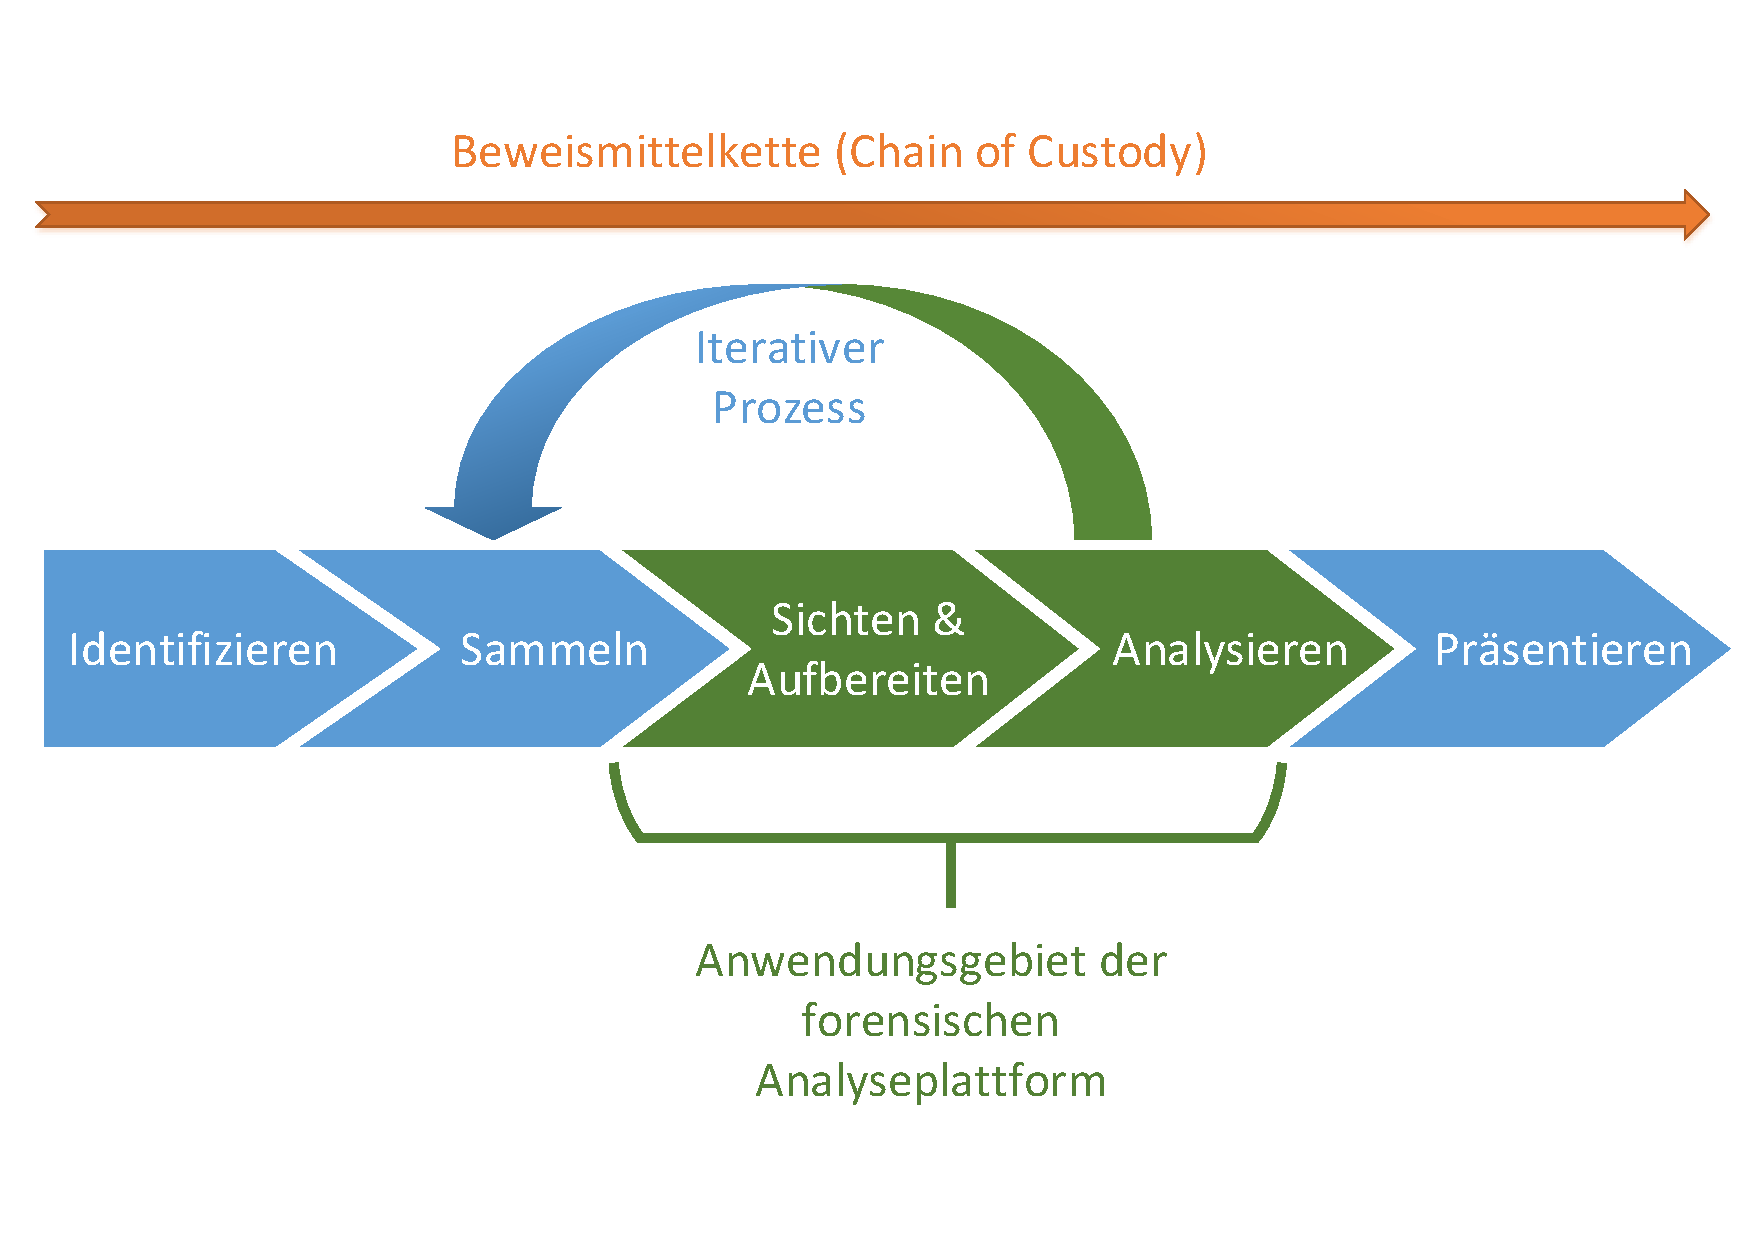
\includegraphics[width=\textwidth]{./resource/digital_forensics_process.pdf}
  \caption{Forensischer Analyseprozess für digitale Beweismittel (Vgl. \cite[S.16]{digital_forensics})}
  \label{fig:digital_forensics_process}
\end{figure}


\noindent
Zu Beginn existiert ein Vorfall oder ein Tatverdacht für eine Straftat. In einem nachfolgenden Schritt ermittelt beispielsweise die Staatsanwaltschaft. Im Ermittlungsverlauf wird darauf der Tatort untersucht oder auch bei Tatverdächtigen nach Hinweisen für die Tat und gegebenenfalls deren Tathergang gesucht. Dieser Schritt beschreibt die Identifikationsphase aus Abbildung \ref{fig:digital_forensics_process}. Hierbei geht es um die Identifikation von möglichen Beweismittel, welche sichergestellt oder  beschlagnahmt werden sollen.\cite[S. 17-24]{digital_forensics}.\\ In der Forensik wird häufig hypothesenbasiert vorgegangen. So entwickelt der Ermittler eine Hypothese, wie eine möglich Straftat begangen wurde und wer diese begangen haben könnte. Darauf aufbauend überlegt er sich welche Spuren für oder gegen diese Hypthese sprechen und welche möglichen Beweismittel eben diese Spuren enthalten könnten (z.B. Kommunikationsdaten auf dem PC oder Bildmaterial auf einem Mobiltelefon).\\

\noindent
Im zweiten Schritt aus Abbildung \ref{fig:digital_forensics_process} geht es um das Vereinnahmen von potentiellen Beweismitteln. Hierbei werden dann die identifizierten Datenträger und Geräte sichergestellt oder beschlagnahmt. In dieser Phase werden beispielsweise auch schon forensisch korrekte Datenträgerabbilder erstellt, auf welchen dann später eine Datenanalyse ausgeführt werden kann.\cite[S. 24-33]{digital_forensics}. In vielen Fällen, beispielsweise bei Unternehmensservern, werden nicht die Geräte selbst sichergestellt sondern nur wichtige Daten forensisch korrekt kopiert. Auch hier findet teilweise schon eine Vorselektion statt, welche Daten benötigt werden und welche Daten im konkreten Fall irrelevant sind.\\

\noindent
Die dritte Phase aus Abbildung \ref{fig:digital_forensics_process} behandelt das Sichten und Aufbereiten der sichergestellten Daten. Gerade bei großen unstrukturierten Datenmengen erfolgt in dieser Phase auch eine Vorselektion, um die Datenmenge nochmals einzugrenzen. Dies kann automatisiert oder auch manuell erfolgen.\cite[S. 33-39]{digital_forensics}. An dieser Stelle beginnt das Anwendungsgebiet der hier entwickelten forensische Analyseplattform. 
So können alle gesammelten Daten in die forensische Analyseplattform importiert und prozessiert werden. Darauf kann über eine allgemeine Suche nach spezifischen Stichworten, Hashsummen oder Zeitpunkten gesucht werden. Dies soll dem Ermittler das Auffinden von fallreleventen Daten erleichtern. Die meisten bekannten forensischen Analysetools bieten ebenfalls Stichwortsuche an, weil eben dadurch große Datenmengen schnell nach bestimmten Kriterien gefiltert werden können.\cite[S. 116-123]{handbook_digital_forensics}\\
In dieser Phase werden aber auch gelöschte, verschlüsselte oder verschleierte Daten wiederhergestellt oder entschlüsselt, sofern dies möglich ist. Eine klassische Methode ist beispielsweise auch das sogenannte \textit{File Carving} auf Datenträgern.\cite[S. 38-39]{digital_forensics}\footnote{Beim File Carving wird versucht logisch zusammenhängende Daten allein anhand des Dateiinhalts zu rekonstruieren, ohne die Dateisystemmetadaten zu nutzen. Die Methode wird gerne angewendet, wenn das Dateisystem nicht wiederherstellbar ist oder wenn gelöschte Dateien auf bereits freigegebenen Speicherbereichen gesucht werden.} Diese Art von Datenaufbereitung beherrscht die hier entwickelte forensische Analyseplattform derzeit noch nicht.\footnote{Es wäre aber durchaus möglich diverse Methoden der Datenaufbereitung zu implementierten. Siehe auch Kapitel \ref{ch:ausblick}.}\\

\noindent
Auch in der anschließenden Analysephase kann die hier entwickelte forensische Analyseplattform genutzt werden (siehe Abbildung \ref{fig:digital_forensics_process}). In dieser Phase werden die aufbereiteten Daten detailliert analysiert, um Informationen zu erhalten die für oder gegen einen bestimmten Tathergang sprechen.\cite[S. 39-45]{digital_forensics} Anhand dieser Informationen werden die eingangs beschriebenen Hypothesen zu möglichen Tathergängen verifiziert. Bei einer Analyse werden aus den Daten komplexe Zusammenhänge und Beziehungen erarbeitet. Beispielsweise werden aus den Rohdaten Kommunikationsverläufe auf Basis von E-Mails oder zeitliche Abläufe basierend auf Zeitstempelanalysen erstellt.\cite[S. 33-39]{digital_forensics}\\
Hierbei geht es auch darum die Aussagekraft eines potentiellen Beweismittels zu ermitteln. So könnte beispielsweise urheberrechtsverletzendes Material auf einem Datenträger eines PCs gefunden werden. Allerdings kann die Aussagekraft dieses potentiellen Beweismittels sehr gering sein, wenn das System bereits durch Schadsoftware kompromittiert wurde.\\
Einige Analyseschritte können automatisiert werden und sind daher prädestiniert für die hier entwickelt Analyseplattform (siehe auch Kapitel \ref{ch:data_processing}).\\

\noindent
Bei der Analyse können auch wieder Verbindungen zu neuen potentiellen Beweismitteln gefunden werden, welchen dann wieder über den forensischen Analyseprozess vereinnahmt und aufbereitet werden. Daher ist der Prozess auch iterativ anzusehen. Gerade durch die Nutzung der forensischen Analyseplattform sollen diese Iterationen verkürzt werden, indem durch die parallelisierte Prozessierung Zeit eingespart werden soll.\\

\noindent
In der letzten Phase des Analyseprozesses müssen die Ermittlungsergebnisse visuell aufbereitet werden, um sie auch vor Gericht präsentieren zu können. Letztlich muss ein Analysebericht erstellt werden, welcher einerseits die Ergebnisse enthält und andererseits nachvollziehbar beschreibt, wie diese Analyseergebnisse zustande gekommen sind.\footnote{Der Bericht sollte so geschrieben sein, dass andere Parteien oder Ermittler die gleichen Ergebnisse reproduzieren können.}\cite[S. 45-47]{digital_forensics}. Viele Analysetools, unter anderem auch das hier genutzt Referenztool \textit{Autopsy}, ermöglichen die semi-automatische Erstellung von Analyseberichten. Die hier entwickelte Analyseplattform kann dies derzeit noch nicht. Bei einer Weiterentwicklung der Analyseplattform wäre diese Funktionalität aber durchaus brauchbar.\\

\noindent
Ein primärer Aspekt bei dem allgemeinen forensischen Analyseprozess aus Abbildung \ref{fig:digital_forensics_process} ist letztlich die Dokumentation der Beweismittelkette. Mit ihr steht und fällt die Aussagekraft der Ergebnisse aus einer forensischen Analyse.\footnote{In der Vergangenheit gab es immer wieder Fälle, bei welchen eine fehlerhaft dokumentierte Beweismittelkette zu sehr fragwürdigen Aussagen auch bei ursprünglich eindeutigen Beweislagen führte.} Daher muss bei der Dokumentation der Beweismittel lückenlos festgehalten werden, was mit letzteren passiert ist. Nachfolgende Liste lieferte hierzu wichtige Kriterien, die festgehalten werden müssen:
\begin{itemize}
\item Die Ermittler, welche das Beweismittel sichergestellt und später analysiert haben.
\item Die Prozesse, Datenaufbereitungen und Analysen, welche durchgeführt wurden.
\item Die Zeitpunkte der Sicherstellung, Aufbereitung und der Analyse.
\item Die Umstände, wie das Beweismittel sichergestellt wurde.
\item Gründe, wieso das Beweismittel sichergestellt wurde.
\item Transportwege und Lagerstätten der Beweismittel.
\item Personen die Zugang zu den Beweismittel hatten und allgemeine Informationen, wie die Beweismittel vor unbefugten Zugriff geschützt wurden.
\end{itemize}

Ein sehr wichtiger Punkt bei der Dokumentation der Beweismittelkette ist Verifikation der Datenintegrität des Beweismittels während des gesamten Analyseprozesses. Dies wird primär durch die Prüfung mittels kryptografischer Hashes erreicht. Letztlich dienen diese zum Schutz vor einer unbeabsichtigten oder beabsichtigten Modifikation des Beweismittels. Das Ändern von Beweismittel oder deren Kopien sollte eigentlich immer vermieden werden. In vielen Fällen ist dies jedoch notwendig, um beispielsweise defekte Datenstrukturen wiederherstellen zu können. Bei solchen bewussten Datenänderungen ist eine entsprechende Dokumentation notwendig.\\ 
Bei der Analyse mit der hier entwickelten Analyseplattform muss auch die Beweismittelkette entsprechend dokumentiert werden. Diese Thematik wird im Rahmen dieser Thesis zumindest in der Theorie nochmals diskutiert. Die derzeitige Implementierung der forensischen Analyseplattform behandelt diesen Aspekt derzeit noch nicht. Aber auch hier könnte in einer Weiterentwicklung eine Beweismittelkette erstellt werden, welche die einzelnen Verarbeitungsprozesse, Zeitpunkte und Nutzerzugriffe dokumentiert.\\



\section{Herkömmliches Analysevorgehen}
\label{sec:common_analysis_approach_part1}
Um die fachlichen Anforderungen an das Analyse-System herauszuarbeiten, soll das herkömmliche Analysevorgehen mit einem vergleichbaren Open-Source Analysewerkzeug betrachtet werden.\\
Die Ausgangslage liefern einige Datenträgerabbilder aus diversen Testszenarien. Diese Datenträgerabbilder sind bezogen auf den forensischen Analyseprozess aus Abbildung \ref{fig:digital_forensics_process} die Grundlage für dir dritte Phase - dem Sichten und Aufbereiten der Daten.

\noindent
Bei gängigen Analysevorgehen werden beispielsweise die Datenträgerkopien mit Betriebssystemprogrammen unter Linux oder mithilfe des Open-Source Analysetools \textit{Autopsy}\footnote{Siehe \url{https://www.sleuthkit.org/autopsy/}. Hierbei wird die Version 4.7.0 in der 64-bit Variante unter Windows 10 Pro genutzt.} unter Windows analysiert. Im kommerziellen Bereich existieren etliche weitere Analyse-Tools mit größerem Funktionsumfang. Nachfolgend wird Autopsy als Referenzsystem unter Windows betrachtet, da es eines der bekanntesten Analysewerkzeuge unter den kostenfreien Open-Source Programmen ist. \\ 

\noindent
Die Datenträgerabbilder können in unterschiedlichen Dateiformaten vorliegen. Mithilfe klassischer Opensource-Tools wie beispielsweise \textit{dd}\footnote{dd ist ein bekanntes Werkzeug zum Kopieren von Daten, welches unter den meisten Unix-basierten Betriebssystemen läuft. Damit können auch ganze Partitionen in einzelne logische Dateien kopiert werden.} kann damit ein Image im sogenannten \textit{RAW}-Format erstellt werden. Von \textit{dd} existiert auch eine forensische Variante \textit{dcfldd} welche beim Kopieren auch noch Hashsummen zur Verifikation berechnet.\cite{linux_forensics}  Andere Tools, wie beispielsweise \textit{FTK-Imager} können auch Datenträgerabbilder in speziellen Container-Formaten erstellen und lesen. Beispielsweise gibt es das \textit{EnCase Physical}-Format mit der Dateiendung \textit{.e01}, oder das \textit{Advanced Forensic Format} mit der Endung \textit{.aff}.\footnote{Siehe \url{https://support.accessdata.com/hc/en-us/articles/222778608-What-Image-Formats-Do-AccessData-Products-Support-}, Stand: 4.4.2018.} Diese Formate unterstützen eine bessere Extraktion von Metadaten oder bieten eine zusätzliche Datenkompression oder Verschlüsselung der darin gespeicherten Dateien an.\cite[S. 35]{digital_forensics}\\

\noindent
Es wird auch unterschieden, ob es sich um ein vollständiges Datenträgerabbild handelt oder um ein logisches Dateiarchiv. Bei dem vollständigen Datenträgerabbilder werden auch nicht allokierte Speicherbereiche innerhalb des Dateisystems, der Partition oder des Datenträgers gesichert. Hier können sich potentiell versteckte und gelöschte Dateifragmente befinden. Auf diesen Datenträgerabbilder kann auch das bereits beschriebene File Carving ausgeführt werden, um gelöschte Dateien wiederherzustellen.\\ 
Ein logisches Dateiarchiv hingegen enthält wirklich nur die Dateien auf einer logischen Ebene und keine unallokierten Speicherbereiche. Von Vorteil hierbei ist eine geringere Speichergröße. Allerdings tritt durch die logische Sicherung ein potentieller Informationsverlust auf, da unallokierte Speicherbereiche nicht berücksichtigt werden, die aber dennoch potentiell auswertbare Informationen liefern könnten. Vertreter logischer Darteiarchive sind die allseits bekannten Archiv-Formate wie beispielsweise ZIP oder TAR.\\

\noindent
Letztlich werden die Beweismittel in unterschiedlichsten Formaten auf dem lokalen Analyse-Rechner gespeichert. Darauf aufbauend können die Daten in spezifische Formate konvertiert werden. Dies hängt aber meistens davon ab, wie sie weiter verarbeitet werden sollen und welche Werkzeuge zu dieser Verarbeitung genutzt werden.\\

\noindent
Im konkreten Testszenario ist das Datenträger-Abbild eines Linux-Rechners im RAW-Format auf dem lokalen Analyse-Rechner gespeichert. Das Abbild selbst kann ein oder mehrere Partitionen enthalten. Innerhalb der Partition werden Daten mithilfe unterschiedlicher Dateisysteme strukturiert gespeichert. Diese Dateisysteme können unter Windows mit dem Werkzeug \textit{X-Mount} oder unter Linux direkt mit dem Befehl \textit{mount} schreibgeschützt gemountet werden. Darauf wird das Dateisystem vom Betriebssystem interpretiert und als logisches Volume auf dem Analyse-Rechner bereitgestellt. Nun können die Dateien mit beliebigen Werkzeugen analysiert werden.\\

\noindent
In der Praxis hat das einfache schreibgeschützte Mounten den Vorteil, dass der Analyst relativ schnell im Dateisystem beliebige Dateien finden und dessen Inhalt mit diversen Tools anzeigen kann. Gerade für eine schnelle Vorprüfung ist dies sinnvoll. Im nachfolgenden Kapitel sollen nun Möglichkeiten zur Speicherung und Aufbereitung des Datenträgerabbildes mithilfe der forensischen Analyse-Plattform untersucht werden.\\

\noindent
Nachfolgend wird nun gezeigt wie ein Datenträgerabbild in einem konkreten Beispiel mit Autopsy (Version 4.7.0 64-bit) unter Windows 10 geöffnet und analysiert wird.\\
Zu Beginn wird bei Autopsy ein neuer Fall erstellt. Hierbei kann ein Name für den Fall angegeben werden und ein Verzeichnis, worin Autopsy die Anwendungsdaten der Analyse speichert. Danach können noch einige optionale Informationen, wie beispielsweise der Bearbeiter, Adressdaten, die Organisation und eine kurze Beschreibung angegeben werden (siehe Abbildung \ref{fig:autopsy_1_case_information}). Bei der Erstellung des Falles wird unter anderem eine neue Falldatenbank angelegt. Diese Datenbanken werden alle lokal auf dem Analyserechner gespeichert.\\

\begin{figure}[ht]
  \centering
  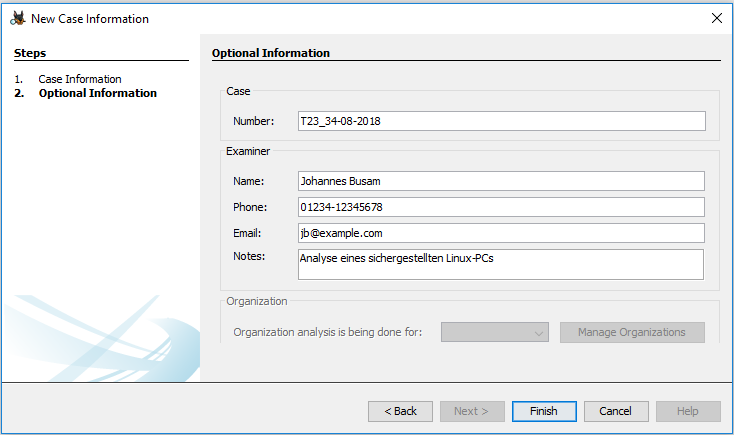
\includegraphics[width=\textwidth]{./resource/autopsy_1_case_information.png}
  \caption{Erstellung eines neuen Falles mit Autopsy}
  \label{fig:autopsy_1_case_information}
\end{figure}

\noindent
Im nächsten Schritt kann nun eine neue Datenquelle dem Fall hinzugefügt werden. Es werden folgende Typen von Datenquellen unterstützt:
\begin{itemize}
\item Ein Datenträgerabbild im \textit{RAW-Format}-Format, Encase-Format oder ein Abbild einer virtuellen Maschine (z.B. von Virtual Box).
\item Ein lokales Laufwerk (z.B. eine externe Festplatte).
\item Logische Dateien aus einem verfügbaren Dateisystem (z.B. ein beliebiger Ordner).
\item Ein Abbild eines beliebigen Speicherbereiches in einer Datei.
\end{itemize}

\noindent
Im konkreten Fall wird ein Datenträgerabbild als Datenquelle hinzugefügt. Dabei muss auch noch eine Zeitzone angegeben werden. Diese Zeitzone kann entscheidend für die Analyse der Zeitstempel auf einem Datenträger sein. In einem \textit{ext}-Dateisystem bei gängigen Linux-PCs werden die Zeitstempel als Anzahl der Sekunden seit dem 1. Januar 1970 in der Zeitzone UTC gerechnet.\cite[S. 326]{filesystem_forensic}\footnote{Diese Zeitdefinition entspricht der sogenannten Unixzeit.} Bei den älteren \textit{FAT}-Dateisystemen hingegen wird die Zeit ohne Zeitzone gespeichert.\cite[S. 192-194]{filesystem_forensic} Je nachdem in welcher Zeitzone das Betriebssystem konfiguriert wurde, welches die Dateien in dem FAT-Dateisystem änderte, ergeben sich zeitliche Unterschiede. Daher muss bei Zeitstempeln auch später bei der Anzeige der Analyseergebnisse immer auch auf die Zeitzone geachtet werden.\footnote{Ein weiteres interessantes Problem ergibt sich auch bei der Sicherung der Beweismittel an einem Tatort. Auch dort ist nie garantiert, dass alle gesicherten Beweismittel überhaupt zeitlich synchronisiert sind. Gerade in Kombination mit Netzwerkverbindungsdaten können bei einer fehlenden Zeitsynchronisation kritische Abläufe zeitlich versetzt sein. Daher muss gerade die Aussagekraft von Zeitstempel immer kritisch betrachtet werden.}\\

\noindent
Im nächsten Schritt können diverse Module zur Datenaufbereitung aktiviert werden. Diese Module dienen zur automatischen Datenaufbereitung und werden ausführlich in Kapitel \ref{sec:common_analysis_approach_part2} beschrieben. In dem Kapitel erfolgt dann auch der Vergleich zur der automatisierten Auswertung mit der hier entwickelten Analyseplattform.\\
Nachdem die entsprechende Module ausgewählt wurden, beginnt Autopsy die Datenquelle zu analysieren. Dies läuft vollständig im Hintergrund ab und der Nutzer kann parallel hierzu die Datenquelle manuell analysieren.\\ 

\noindent
Das Importieren einer Datenquelle bei Autopsy besteht letztlich aus dem Erstellen eines Falls und der Angabe einiger Konfigurationsmöglichkeiten. Die eigentliche Datenquelle wird hierbei nicht in einen internen Anwendungsordner kopiert sondern wird während der Analyse auf dem Rechner bereitgestellt (entweder als Datenträgerabbild oder direkt als externer Datenträger). In den Anwendungsordner selbst werden Metainformationen, wie beispielsweise die Indexierung bestimmter Daten, abgespeichert um während der Analyse schneller darauf zugreifen zu können. Prinzipiell ist dieses Vorgehen sehr gut, da der Ermittler direkt mit der Arbeit beginnen kann und keine Daten mehr kopieren muss.\footnote{Das Erstellen eines Datenträgerabbildes aus dem originalen Asservat wurde hierbei schon vorher durchgeführt.}

\section{Umsetzung in der Hadoop Analyse-Plattform}

Im vorangegangen Kapitel wurde bereits beschrieben, wie bei Autopsy Datenträgerabbilder als sogenannte Datenquellen in die Analysesoftware importiert werden. Wie erwähnt wird das Datenträgerabbild oder der extern angeschlossene Datenträger nicht in einen internen Anwendungsordner kopiert. Autopsy arbeitet direkt auf den Daten um ein unnötiges Kopieren von Daten und dessen Ressourcenaufwand zu vermeiden. \\

\noindent
Im Vergleich hierzu arbeitet die hier entwickelte forensische Analyseplattform auf einem eigenen Computer-Cluster basierend auf mehreren Knoten und nicht nur auf einem einzelnen Analyserechner. Daher müssen die forensisch relevanten Daten zuerst über das Netzwerk in die Analyseplattform importiert werden. \\
Da die Analyseplattform auf dem Hadoop-Framework aufbaut, bildet der Kern der Datenspeicherung das Hadoop Distributed File System (HDFS)\footnote{Sieh auch Kapitel \ref{sec:theory_hdfs}.}. Hierbei geht es nicht nur darum, wie die Daten im Hadoop-Framework verwaltet werden, sondern vielmehr um die Art und Weise, wie Daten forensisch korrekt gespeichert werden können.\\


\noindent
Zur Speicherung der Daten des Datenträgerabbildes im Hadoop-Framwork gibt es mehrere Möglichkeiten, deren Vor- und Nachteile nachfolgend dargestellt werden sollen.

\subsection{Variante 1 - Datenträgerabbild im HDFS speichern}
\label{subsec:variant1}

Die naheliegende Variante zur Speicherung der Beweismittel, wäre die Datenträgerabbilder direkt im HDFS abzuspeichern. Allein die Größe der Abbilder wäre nicht problematisch. Um eine entsprechende Aufteilung kümmert sich das HDFS. Allerdings hat die Lösung den entscheidenden Nachteil, bei der Weiterverarbeitung der Daten.\\ 

\noindent
Auf Betriebssystemebene können solche Datenträger mit mehreren Partitionen und unterschiedlichen Dateisystemen interpretiert und eingebunden werden. Dabei liegen die Dateien als fragmentierte Blöcke in einer spezifischen Datenstruktur vor, welche das Dateisystem des Abbildes beschreiben. Je nachdem, ob ein Datenträgerabbild direkt von einer Partition eines Datenträgers oder vom ganzen Datenträger erstellt wurde, sind in dem Abbild unter Umständen auch mehrere Partitionen samt Partitionstabelle enthalten. Von diesen Partition kann wiederum jede einzelne Partition ein eigenes Dateisystem, wie beispiels FAT, ext4, oder NTFS enthalten. Dieses Dateisystem enthält dann die eigentlichen Dateien, welche logisch zusammengesetzt werden müssen.\\ 
Viele Betriebssysteme bieten hier bereits eine weitreichende Unterstützung zum Lesen und Schreiben dieser Dateisysteme. Hierzu können die Dateisysteme einzelner Partitionen des Datenträgerabbildes \textit{gemountet} werden.\\

\noindent
Aber innerhalb des Hadoop-Frameworks findet sich keine Unterstützung zum Lesen von beliebigen Dateisystemen. Denn normalerweise nutzen JAVA-Applikationen ein definierte Schnittstelle auf Basis von Dateien, die wiederum vom Betriebssystem bereitgestellt werden. Um die logischen Dateien aus dem Datenträgerabbild extrahieren zu können, müsste für jedes einzelnes Dateisystem eine eigene Implementierung in Java geschrieben werden. Und diese Implementierung müsste dann auch noch für das HDFS-Dateisystem optimiert sein.\\ 

\noindent
Darüber hinaus wäre das Extrahieren der Dateien aus einem Dateisystem auf einem Datenträgerabbild auch nicht wirklich performant. Angenommen das Auslesen würde mit Apache Spark durchgeführt werden. Aufgrund der eingangs beschriebenen Datenlokalität (siehe Kapitel \ref{ch:theory_hadoop}) wären auf jedem Knoten einzelne Blöcke von beispielsweise 128 MB Größe vorhanden. Um dann im ext4-Dateisystem eine Datei lesen zu können, sollten zumindest die Dateisystemmetadaten verfügbar sein. Darüber hinaus kann der Dateiinhalt einer einzelnen Datei verstreut innerhalb des Dateisystems liegen. Je nach Grad der Fragmentierung des Dateisystems, müsste dann auf einem Data-Node innerhalb des Clusters schlimmstenfalls dutzende weitere Blöcke anderer Knoten nachgeladen werden, um den Inhalt einer einzelnen Datei zu verarbeiten. Dies würde das Prinzip der Datenlokalität aushebeln. Abbildung \ref{fig:ext4_to_hdfs} skizziert diese verstreute Aufteilung einer Datei im physikalischen Hadoop-Cluster.\\ 
\begin{figure}[ht]
  \centering
  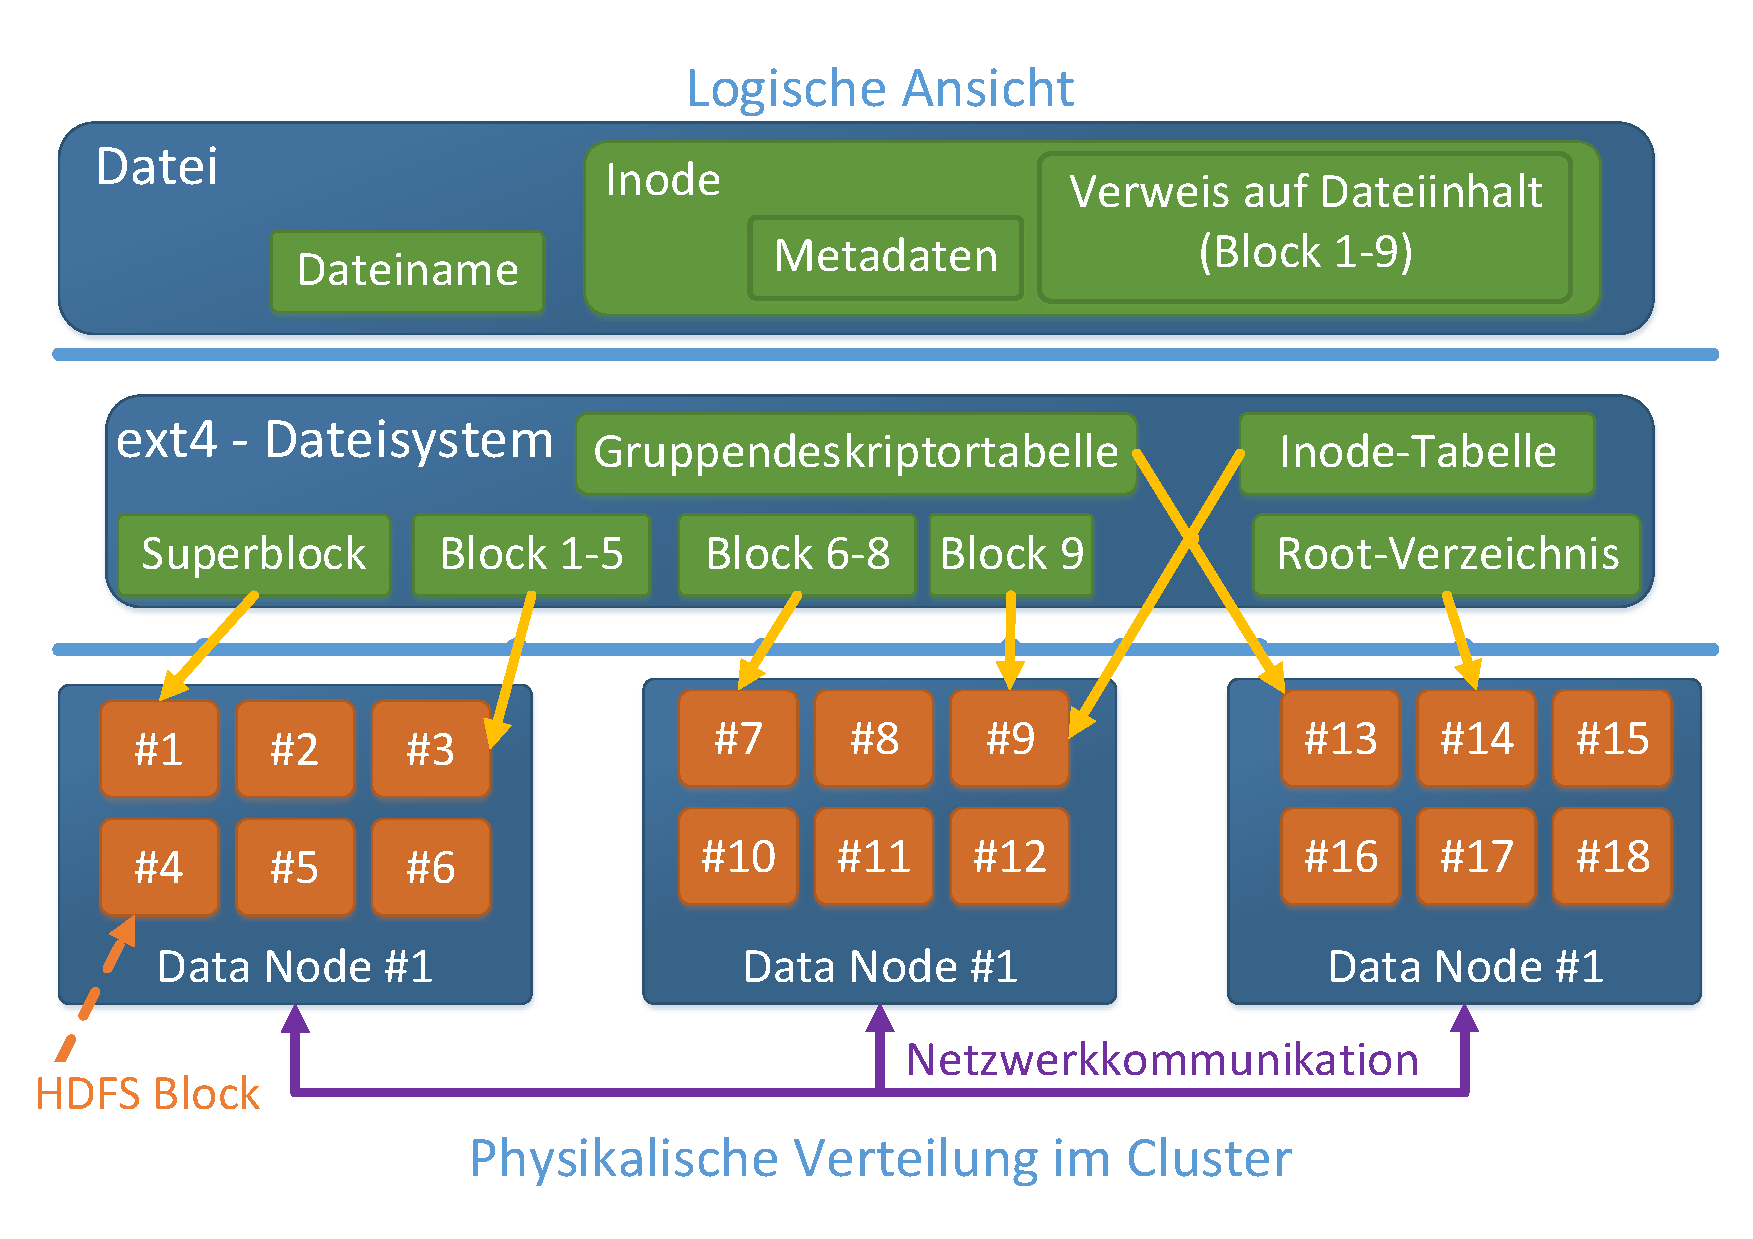
\includegraphics[width=\textwidth]{./resource/ext4_to_hdfs.pdf}
  \caption{Aufteilung der Daten des Datenträgerabbildes im Hadoop-Cluster}
  \label{fig:ext4_to_hdfs}
\end{figure}

\noindent
Das Abbild zeigt eine Datei, welche aus logischer Sicht einen Dateinamen, Metadaten (beispielsweise Zugriffsrechte) und einen Inhalt besitzt. Der Inhalt ist in 9 Blöcken zu jeweils 2048 Byte aufgeteilt.\footnote{Die Blockgröße wird hierbei vom Ext4-Dateisystem bestimmt und ist die kleinste allozierbare Einheit im Dateisystem. In der physikalischen Aufteilung im HDFS Dateisystem gibt es auch Blöcke, welche aber beispielsweise eine Größe von 128 MB aufweisen (orange in Abbildung \ref{fig:ext4_to_hdfs}).} Um nun den Inhalt aus dem ext4-Dateisystem einer Datei auszulesen. Wird zuerst der Superblock benötigt. Dieser enthält allgemeine Informationen zum Dateisystem. Darauf wird die Gruppendeskriptortabelle benötigt, um auf einzelne Blockgruppen zuzugreifen.\footnote{Das Dateisystem selbst in mehrere autarke Bereiche unterteilt, welche für sich genommen eigenständig Daten einer Teilmenge aller Dateien vorhalten. Dies sind die sogenannten Blockgruppen.} Über eine Blockgruppe kann wiederum auf die Inode-Tabelle zugegriffen werden. Diese speichert die Metadaten einzelner Dateien als sogenannte \textit{Inodes} ab. Ein Inode-Eintrag hält wiederum Verweise auf die Blöcke, welche den Dateiinhalt beschreiben. Der Dateiname ist wiederum in dem logisch übergeordneten Verzeichnis gespeichert. Das oberste Verzeichnis, ist das Wurzelverzeichnis. Dieses enthält die Namen der Kind-Dateien und entsprechende Verweise zum Inode.\\
Beim Auslesen einer Datei müssen nun etliche Speicherstellen innerhalb des Dateisystems gelesen und interpretiert werden. Angenommen, dass ein konkretes ext4-Dateisystem in einer 100 GB großen Partition gespeichert wird, so wir diese große Datei im HDFS-Dateisystem in 800 große Blöcke zu je 128 MB aufgeteilt und auf den einzelnen Knoten des Clusters gespeichert. Hierbei kann aber kein Einfluss darauf genommen werden, wo welche Blöcke mit welchem Inhalt gespeichert werden. Letztlich bedeutet dies wiederum, wenn in einem Apache Spark Executor zu Verarbeitung der Daten eine Datei des Knotens gelesen werden soll, müssen schlimmstenfalls etliche Datenblöcke von anderen Knoten angefordert werden. Dieses Problem wird in Abbildung \ref{fig:ext4_to_hdfs} ersichtlich. Dort werden die benötigten Daten zum Auslesen der einen logischen Datei auf drei unterschiedlichen Data Nodes gespeichert. Und dadurch wird auf Netzwerkebene unnötig viel Last erzeugt. Letztlich gilt für das Prinzip der Datenlokalität, dass die einzelnen Blöcke im HDFS möglichst unabhängig von einander verarbeitet werden können. Diese Problematik trifft übrigens nicht nur bei der Ext-Dateisystemfamilie auf sondern auch bei anderen Dateisystemen.\\

\noindent
Aus den oben genannten Gründen ist die Speicherung von Datenträgerabbilder als eine einzige logische Datei im HDFS nicht geeignet für die Analyse im Hadoop-Cluster.

\subsection{Variante 2 - Logische Dateien im HDFS speichern}
In dieser Variante wird das Beweismittel auf dem lokalen Analyserechner gemountet. Darauf aufbauend werden alle Dateien auf logischer Ebene direkt in das HDFS importiert. Damit ist die gesamte Dateisystemstruktur aus dem Datenträgerabbild im HDFS abgelegt. Einzelne Dateien aus dem Datenträgerabbild sind nun auch als einzelne Dateien im HDFS gespeichert und können unabhängig voneinander prozessiert werden. Darüber hinaus ist die Datenstruktur im HDFS unabhängig von dem Dateisystem des importierten Datenträgerabbildes.\\
Damit sind die Nachteile der vorangegangen ersten Variante aus Kapitel \ref{subsec:variant1} behoben. Allerdings ist das bereits erwähnte File Carving, beziehungsweise das Auffinden von gelöschten Dateien nun nicht mehr im Hadoop-Framework möglich. Denn bei dieser Variante werden ja nur die Dateien aus dem Dateisystem in das Hadoop-Framwork importiert und nicht allokierte Speicherbereiche werden nicht weiter untersucht. Theoretisch wäre es aber auch möglich zusätzlich das vollständige Datenträgerabbild in das HDFS zu importieren, um dann später freie Speicherbereiche analysieren zu können. Im Rahmen dieser Thesis wird diese Einschränkung jedoch vorerst akzeptiert. Eine File Carving ist daher mit der hier entwickelten forensischen Analyseplattform noch nicht möglich. Andererseits können nun in Analogie zur Referenzsoftware Autopsy auch beliebige Verzeichnisse als Datenquelle in die Analyseplattform geladen werden.\footnote{Siehe Kapitel \ref{sec:common_analysis_approach_part1}.}\\ 

\noindent
Interessant an dieser Variante ist das Verhalten des HDFS-Dateisystems bezüglich der Metadaten und der unterschiedlichen Größen von Dateien. Zur Analyse der Dateien auf dem Datenträger werden auch die Metadaten zu den Dateien benötigt. Beim Importieren muss darauf geachtet werden, dass alle Metadaten des lokalen Dateisystems im Datenträgerabbild unverändert in das HDFS kopiert werden. Im HDFS werden auch Metadaten zu den einzelnen Dateien gespeichert. Möglicherweise könnten diese Dateiattribute wiederverwendet werden, um die Metadaten aus dem originalen Dateisystem zu speichern.
Welche Metadaten bereits im HDFS mit angelegt werden, zeigt Abbildung \ref{fig:hdfs_file_properties} anhand eines Ausschnitts aus der Web-Repräsentation eines HDFS.\\
%TODO Abbildung prüfen. Die Darstellung ist zu klein!!! 
\begin{figure}[ht]
  \centering
  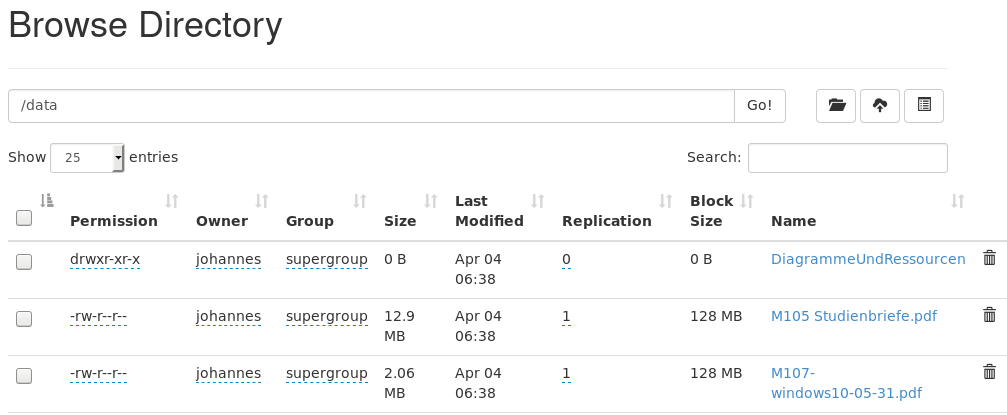
\includegraphics[width=\textwidth]{./resource/HDFS_FS_Example.png}
  \caption{HDFS - Dateieigenschaften}
  \label{fig:hdfs_file_properties}
\end{figure}

\noindent
Daraus ist ersichtlich, dass jede Datei entsprechende Dateirechte hat und einem Nutzer und einer Gruppe zugeordnet ist. Zusätzlich wird die Größe und der Zeitstempel der letzten Änderung gespeichert.\footnote{Bei Dateiverzeichnissen ist die Größe 0 Byte.} Die Anzahl der Replikationen und die Blockgröße sind spezifisch für das HDFS. Jede Datei kann auf einer unterschiedlichen Anzahl von Knoten repliziert sein. Die Standardkonfiguration definiert 3 Replikationen im realen Cluster, wobei Verzeichnisse nur logisch auf dem Name Node abgelegt werden und damit auf keinem DataNode explizit repliziert werden. Auch die Blockgröße ist in der Standardkonfiguration auf 128 MB festgelegt. Wie im Grundlagenkapitel \ref{sec:theory_hdfs} erwähnt, werden die Dateien in mehren Blöcken zu maximal 128 MB gespeichert und auch repliziert.\footnote{Diese Blockgröße kann aber konfiguriert werden.}\\
Bezogen auf klassische Dateisysteme entspricht ein Block im HDFS einem Block im Ext4-Dateisystem oder einem Cluster im NTFS-Dateisystem. Es ist letztlich die kleinste allozierbare Dateneinheit im Dateisystem.\cite[S.129-140]{filesystem_forensic} Dies bedeutet allerdings nicht, dass für jede Datei im HDFS auf den jeweiligen Data Nodes immer mindestens 128 MB Speicher belegt werden. Denn die reale Speicherbelegung auf dem Data Node beschränkt sich auch auf die reale Größe der Datei im lokalen Dateisystem des Data Nodes.\cite[S. 16-17]{professional_hadoop}\\

\noindent
Mit dem Befehl aus Listing \ref{lst:hdfs_put_command} können Dateien von einem lokalen Verzeichnis in das HDFS importiert werden. 
\begin{lstlisting}[label={lst:hdfs_put_command},caption= Befehl zum Speichern einer Datei im HDFS,captionpos=b,frame=single,style=customshell]
# hdfs dfs -put [source] [destination]
hdfs dfs -put test.pdf /test.pdf
\end{lstlisting}

\noindent
Hierbei werden die ursprünglichen Metadaten der Datei nicht übernommen. So beschreibt der oben erwähnte Modifikationszeitstempel den Zeitpunkt, zu dem die Datei im HDFS das letzte Mal geändert wurde. Dies entspricht initial dem Import-Zeitpunkt. Auch werden Nutzer und Gruppenrechte nicht übernommen. Prinzipiell wäre es aber möglich die Metadaten aus dem lokalen Dateisystem mit in das HDFS zu übernehmen.\footnote{Hierzu kann dem \textit{put}-Befehl aus Listing \ref{lst:hdfs_put_command} der Parameter \textit{-p} mit übergeben werden.} Ratsam ist dies jedoch nicht, da der Nutzer, die Gruppe und die dazugehörigen Zugriffsrechte in einem produktiven HDFS-Cluster verwendet werden, um Zugriffsbeschränkungen einzelner Nutzer und Anwendungen auf Dateien im HDFS umzusetzen. Die Metadaten des originalen Dateisystems sollten daher mit einer anderen Methode im HDFS gespeichert werden.\\

\noindent
Eine bessere Möglichkeit bietet das HDFS mithilfe von erweiterten Dateiattributen. Diese können beliebige Informationen zu einer Datei speichern. Mit nachfolgenden Befehlen kann beispielsweise der Zeitstempel der Erstellung einer Datei aus dem ursprünglichen Dateisystem im HDFS als erweitertes Attribut gespeichert und ausgelesen werden. Hierbei kann der Name des Attributs (\textit{user.ntfs.creationtime}) und dessen Inhalt (\textit{2018-04-07T11:14:42,798583789+02:00}) frei gewählt werden.
\begin{lstlisting}[label={lst:hdfs_fattr_command},caption= Befehl zum Hinzufügen und Auslesen von Metadaten,captionpos=b,frame=single,style=customshell]
# Create custom file attribute
hdfs dfs -setfattr -n user.ntfs.creationtime -v "2018-04-07T11:14:42,798583789+02:00" /test.pdf

# Read custom file attribute
hdfs dfs -getfattr -d -n user.ntfs.creationtime /test.pdf
\end{lstlisting}

\noindent
Mit dem obigen Befehl ist es also prinzipiell möglich, alle Metadaten des ursprünglichen Dateisystems als erweiterte Dateiattribute im HDFS zu speichern. Allerdings müssen diese Metadaten zur Weiterverarbeitung zuerst für jede Datei im HDFS eingetragen werden.\\
Zusätzlich müssen beim Verarbeiten der Daten mit Apache Spark die Metadaten auslesbar sein. Dieses Auslesen ist umständlich aber möglich.\footnote{Siehe Metadaten-Extraktion im Projekt \textit{foam-processing-spark} unter \url{https://github.com/jobusam/foam-processing-spark}.}\\

\noindent
Es gibt jedoch zwei entscheidende Nachteile bei dieser Variante die beide den gleichen Ursprung haben. 
Der erste Nachteil ist, dass jede einzelne Datei aus dem ursprünglichen Dateisystem als getrennte eigenständige Datei in das HDFS hochgeladen werden muss. In einem einzigen Dateisystem können Millionen kleine Dateien gespeichert sein, die alle auch in das HDFS importiert werden müssen. Allerdings ist das HDFS primär für größere Dateien (in der Größenordnung einer Blockgröße von 128 MB) ausgelegt und kann viele kleine Dateien nicht wirklich effizient speichern und bereitstellen. Dies ist dem Umstand geschuldet, dass alle Metadaten auf dem Name Node gespeichert werden und nur der Dateiinhalt im Cluster aufgeteilt wird.\cite[S. 16]{professional_hadoop} Wenn nun viele kleine Dateien gespeichert werden, dann steigt der Speicherverbrauch im NameNode an und beeinträchtigt die Performanz des Systems. Der zweite Nachteil verstärkt dieses Problem. Denn wenn nun auch noch die Metadaten aus dem ursprünglichen Dateisystem als erweiterte Metadatenattribute im HDFS gespeichert werden, dann benötigt der Name Node noch mehr Ressourcen. Darüber hinaus wäre beispielsweise die Verarbeitung der Metadaten mit Apache Spark nur bedingt parallelisierbar, da diese Daten immer zuerst an dem einen Name Node angefordert und über das Netzwerk zu den einzelnen Spark Executoren gesendet werden müssten. Erst dann könnten letztere Executoren die Daten parallel verarbeiten. Abbildung \ref{fig:storage_hdfs_extended_attributes} skizziert nochmals den Datenfluss bei dieser Lösung.\\

\begin{figure}[ht]
  \centering
  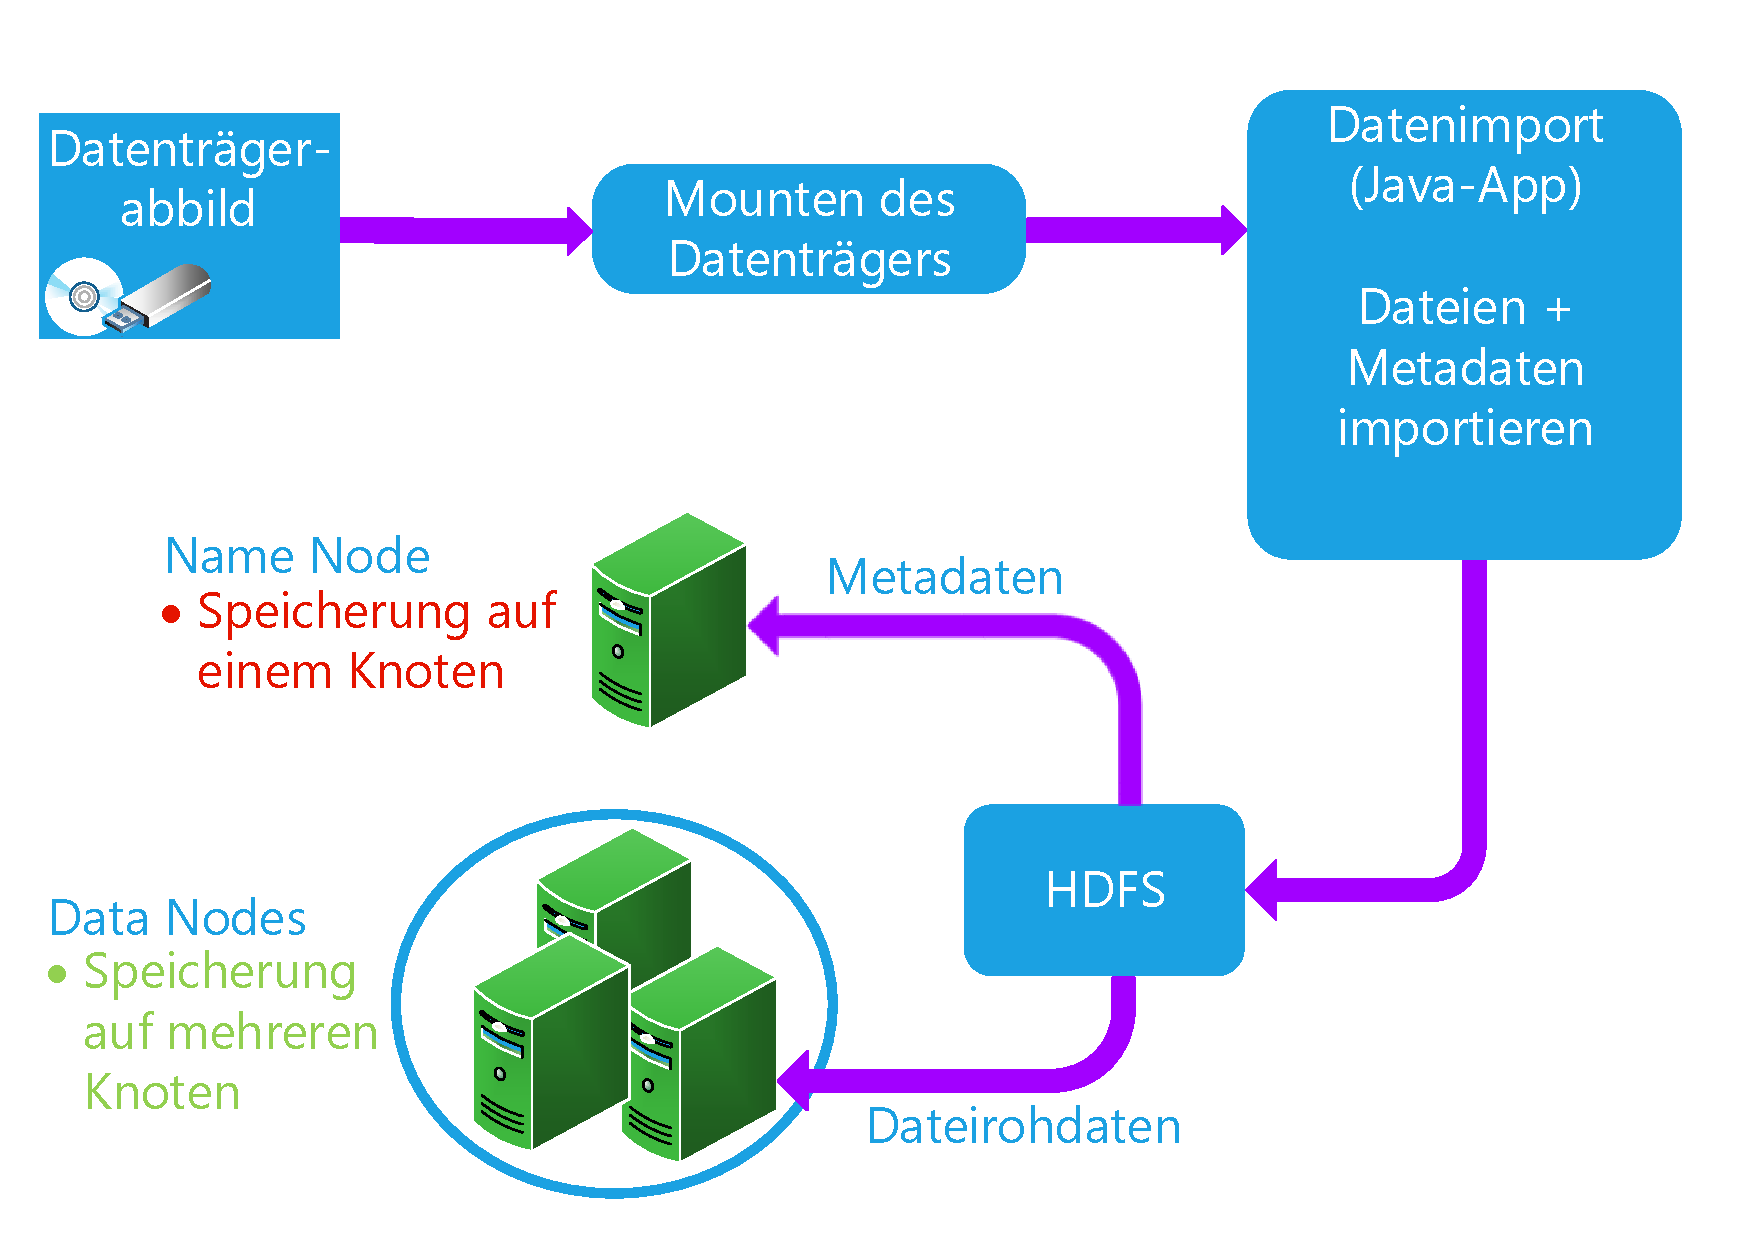
\includegraphics[width=\textwidth]{./resource/storage_hdfs_extended_attributes.pdf}
  \caption{Datenspeicherung mit erweiterten Dateiattributen im HDFS}
  \label{fig:storage_hdfs_extended_attributes}
\end{figure}

\noindent
Das Fazit der Variante 2 lautet daher, dass die Dateimetadaten des originalen Datenträgerabbildes höchstens als erweiterte Attribute im HDFS abgelegt werden könnten. Beim Importieren müssten diese Metadaten bei jeder einzelnen Datei explizit nachgetragen werden. Nicht zuletzt werden alle Datei-Metadaten physikalisch im Name Node gespeichert. Dadurch benötigt der Name Node mehr Speicher und könnte zu einem Flaschenhals im System werden. Zudem wäre die parallelisierte Datenverarbeitung eingeschränkt, da die Metadaten immer zuerst von dem Name Node angefordert werden müssen. Aus diesen Gründen ist die Variante 2 nicht akzeptabel. 

\subsection{Variante 3 - Speicherung in Dateicontainer}

Die vorangegangene Variante überzeugt nicht, da die Speicherung vieler kleiner Dateien nicht effizient im HDFS durchgeführt werden kann. Da alle Metadaten einer Datei im Name Node abgelegt werden, bildet der Name Node bei vielen kleinen Dateien ein Flaschenhals. Zur Lösung dieser Problematik existieren im Hadoop-Umfeld diverse Dateicontainer. Diese Dateicontainer können mehrere Dateien in einem strukturierten Format speichern. In Analogie zu bekannten Dateicontainern, wie beispielsweise \textit{ZIP}-Archiven oder \textit{TAR}-Archiven existieren im Hadoop-Umfeld \textit{Sequence Files}, \textit{RC/ORC Files}, \textit{Avro-Files} oder \textit{Parquet-Files}.\cite[S. 296]{expert_hadoop_admin} \\
Das Hauptziel dieser Dateiformate ist viele kleine Daten auch auch Dateien in größere Dateien zu speichern, um eine bessere Parallelisierung und eine effiziente Speicherung in Hadoop zu ermöglichen. Oftmals unterstützen diese Formate auch eine Datenkompression, um gegebenenfalls Speicherplatz sparen zu können. Viel wichtiger ist jedoch die Teilbarkeit dieser Dateiformate. Wie bereits beschrieben, werden Dateien im HDFS in größere Blöcke geteilt und im HDFS auf unterschiedlichen Knoten gespeichert. Innerhalb eines Blocks muss es also möglich sein, einzelne Einträge beziehungsweise Datensätze lesen zu können. Die oben erwähnten Hadoop Dateiformate unterstützen eben diese Teilbarkeit.\footnote{Im Gegensatz hierzu sind beispielsweise die meisten Dateisysteme in einer Partition eben nicht teilbar. Denn wenn ein Block in der Mitte des Dateisystems ausgelesen werden soll, so können die Daten nicht ohne die Dateisystemmetadaten interpretiert werden. Daher ist auch die erste Variante aus Kapitel \ref{subsec:variant1} eben nicht im HDFS anwendbar.}\\

\noindent
Nachfolgend soll das \textit{Sequence File}-Format in Abbildung \ref{fig:sequence_file_format} näher betrachtet werden.\footnote{Siehe auch \cite[S. 134]{hadoop_definitive_guide} und \url{https://hadoop.apache.org/docs/r2.7.5/api/org/apache/hadoop/io/SequenceFile.html}, Stand 18.8.2018.}

%TODO Beim Header ist die linke Linie nicht an der unteren linken Ecke!
\begin{figure}[ht]
  \centering
  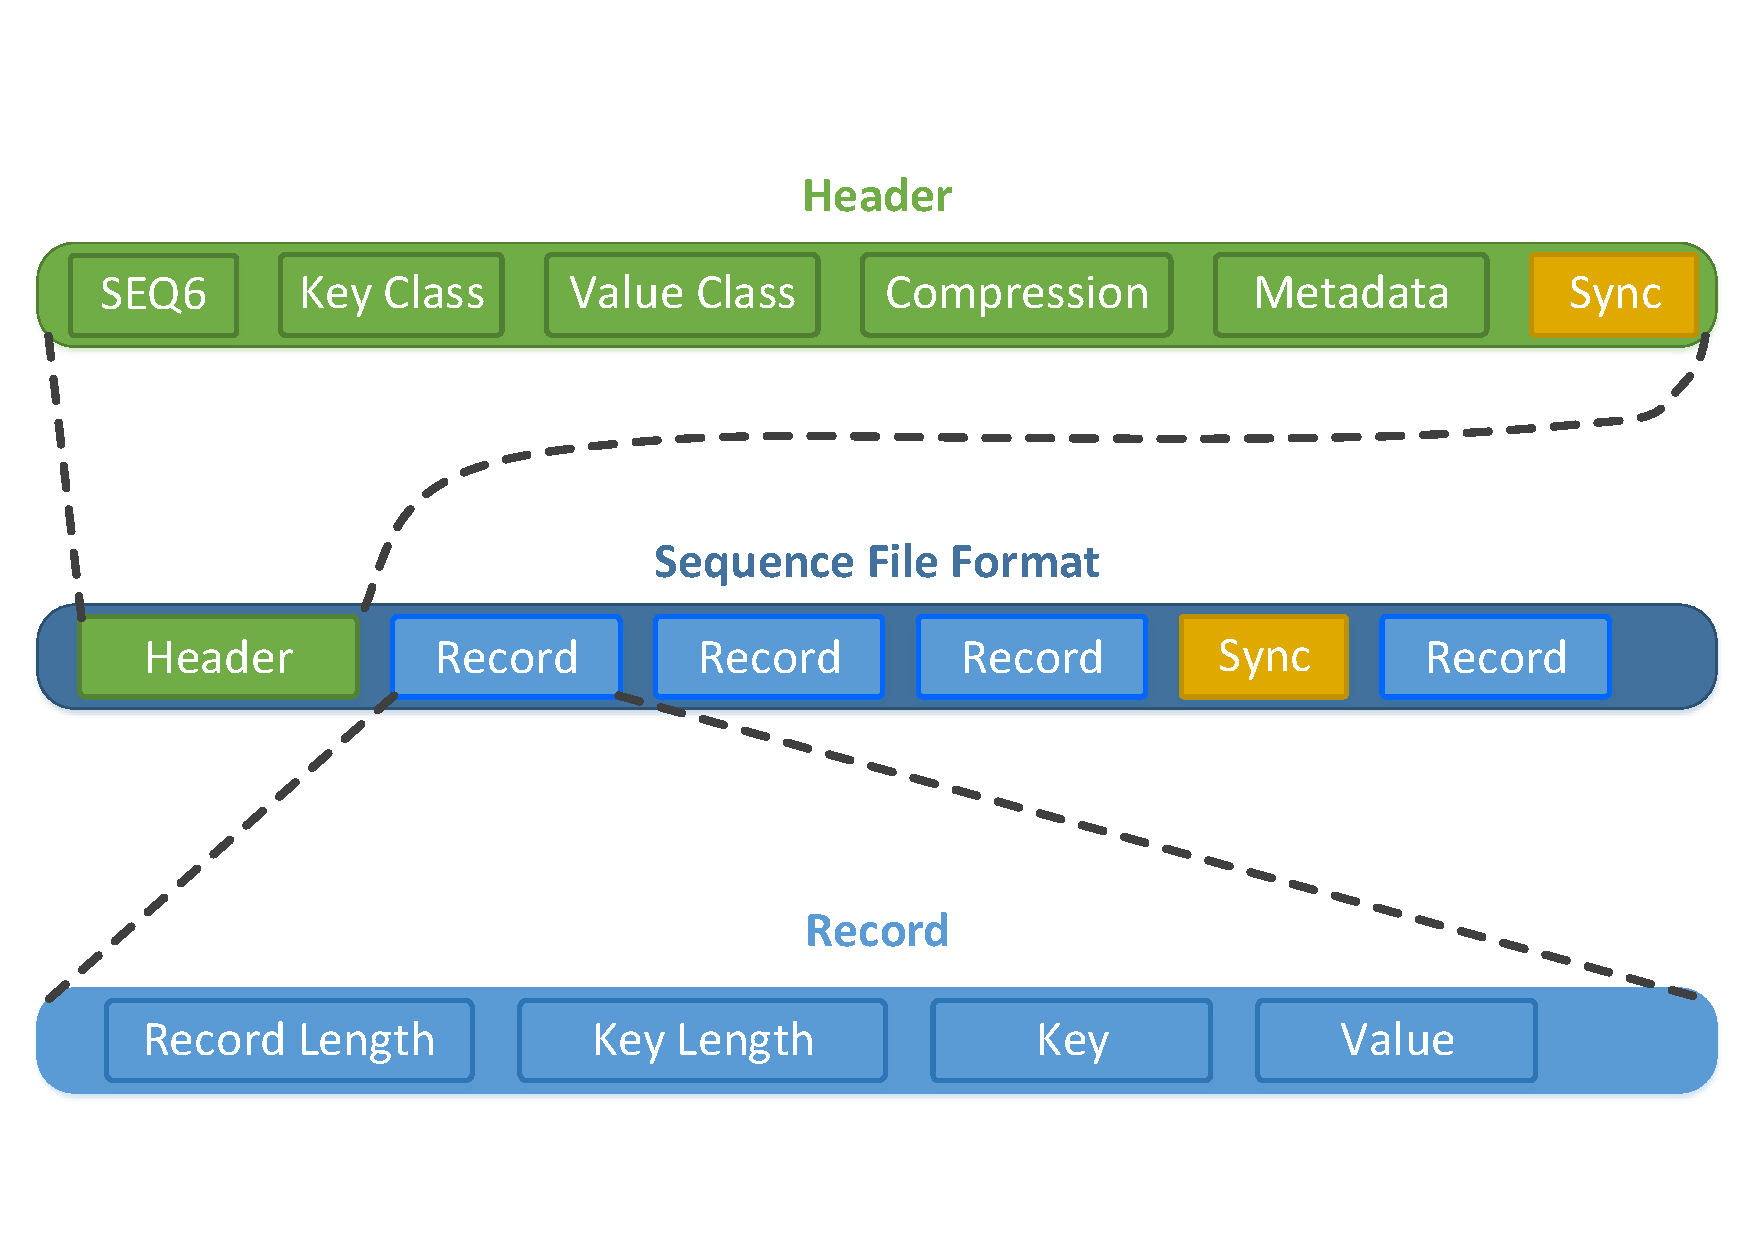
\includegraphics[width=\textwidth]{./resource/sequence_file_format.pdf}
  \caption{Sequence File Format (Vgl. \cite[S. 134]{hadoop_definitive_guide})}
  \label{fig:sequence_file_format}
\end{figure}

\noindent
Das Sequence File Format besteht aus einem Header und mehreren Einträgen. Diese Einträge wiederum sind eigenständige Schlüsselwertpaare, welche die eigentlichen Daten beinhalten. Ein Schlüsselwertpaar,in Abbildung \ref{fig:sequence_file_format} auch \textit{Record} genannt, enthält einen eindeutigen Schlüssel (\textit{Key}) und einen Inhalt (\textit{Value}). Zusätzlich wird am Anfang die Gesamtlänge des Schlüsselwertpaares und die Länge des Schlüssels in Bytes angegeben. Damit ist es möglich den Schlüssel sowie den Inhalt innerhalb des Sequence Files zu bestimmen. Allerdings ist dadurch noch nicht klar, wie der Schlüssel oder Inhalt zu interpretieren ist. Daher sind im Header des Sequence File Formats jeweils die Namen der Java-Klassen in den Feldern \textit{Key Class} und \textit{Value Class} gespeichert, die den Datentyp definieren.  
Im Header befinden sich auch Informationen, ob und in welcher Form eine Datenkompression auf die Daten angewendet wurde.\\
Zuletzt werden in unregelmäßigen Abständen sogenannte Sync-Felder abgespeichert. Diese dienen zur Unterstützung der eingangs erwähnten Teilbarkeit des Dateiformats. Eine Anwendung kann sich mithelfe der Sync-Felder von einer beliebigen Stellen aus innerhalb der Datei auf den Anfang eines Schlüsselwertpaares synchronisieren. Damit können auch Schlüsselwertpaare aus einem beliebigen HDFS-Block interpretiert werden.\footnote{Voraussetzung hierbei ist allerdings, dass die Anwendung vorher schon die Datentypen der Schlüsselwertpaare kennt.}\\ 

\noindent
Prinzipiell können damit sehr kleine Dateien (z.B. kleiner 10 MB) in mehrere Sequence Files strukturiert im HDFS gespeichert werden. Diese Variante enthält aber noch einige Hindernisse. Zuerst stellt sich hier die Frage, wie diese Sequence Files erstellt werden sollen. Hierbei müsste die Anwendung zum Datenimport auf dem Analyse-Rechner die Sequence Files zuerst lokal auf dem Rechner erstellen und danach in das HDFS hochladen. Gegebenenfalls müssten diese Sequence Files sogar noch auf dem lokalen Rechner persistent zwischengespeichert werden. Die Datenimport-Anwendung würde entsprechen mehr Ressourcen benötigen.\\
Ein interessanteres Problem ist aber die Datenverarbeitung im HDFS. Angenommen es existieren nun Sequence Files mit den Dateiinhalten und den Metadaten in den Dateien. 
Mit Apache Spark können diese Sequence Files gelesen werden und beispielsweise die Hashsummen und die Medientypen ermittelt werden.\footnote{Siehe auch Kapitel \ref{ch:data_processing}.} Allerdings müssten beim Schreiben die Daten in neue Sequence Files geschrieben werden. Denn im HDFS ist es nicht möglich existierende Dateien wahlfrei zu modifizieren.\cite[S. 42]{expert_hadoop_admin} Es können maximal neue Daten an das Dateiende einer Datei geschrieben werden. Damit müssten bei der Datenverarbeitung nochmals alle Daten neu geschrieben werden. Dies führt zu unnötigem Ressourcenverbrauch. Andererseits könnten die Rohdaten und die Metadaten in getrennte Sequence Files gespeichert werden. Damit müssten dann nur Sequence Files mit den Metadaten neu geschrieben werden. Es wäre auch denkbar alle neu gewonnen Metadaten in eigenständige neue Sequence Files zu schreiben.\\ 
Allerdings könnte dies wiederum zu einer Art von Fragmentierung von logisch zusammenhängenden Daten führen. Denn nun sind die Metadaten und Rohdaten in mehrere Sequence Files aufgeteilt. Schlimmstenfalls könnten dadurch die Metadaten und Rohdaten, welche eine logische Datei repräsentieren, auf unterschiedlichen Knoten im Hadoop-Cluster liegen. Dies würde das Prinzip der Datenlokalität in gewissem Maße beeinträchtigen. Dies hängt aber auch stark davon ab, wie die Daten für die Verarbeitung angefordert werden. Ist es notwendig die Metadaten und die Rohdaten einer logischen Datei gemeinsam zu verarbeiten, oder können diese auch unabhängig voneinander auf getrennten Knoten prozessiert werden?\\

\noindent
Zusammengefasst ist diese Variante technisch möglich. Allerdings besteht eben diese Problematik beim Speichern von neu gewonnen Informationen. Letztlich ist es durchaus sinnvoll wenn die Rohdaten, die originalen Metadaten aus dem ursprünglichen Dateisystem und die neu gewonnenen Metadaten bei der Datenanalyse für eine logische Datei auch physikalisch zusammen gespeichert werden.\footnote{Zumindest sollten die Daten auf dem gleichen Knoten liegen, um Netzwerkverkehr zu vermeiden.}\\ 
Ein anderer Aspekt ist auch die Komplexität der Anwendung. Bei der praktischen Implementierung dieser Variante müsste immer betrachtet werden, wo nun welche Informationen liegen und wie letztlich alle Informationen zu einer Datei aus den Sequence Files zusammengesetzt werden müssen. Meiner Ansicht nach wäre die Implementierung hierbei schon entsprechend komplex. Darüber hinaus sollen ja nur kleine Dateien in Sequence Files abgelegt werden. Große Dateien hingegen könnten ja direkt im HDFS gespeichert werden. Dies würde die Anwendungskomplexität weiter erhöhen. Daher überzeugt auch diese Variante nicht zur Datenspeicherung.\footnote{Diese Entscheidung, diese Variante nicht zu verfolgen, basiert nur auf den theoretischen Vorüberlegungen. Auf eine prototypische Implementierung dieser Variante wurde verzichtet, weil mit der vierten Variante zur Datenspeicherung ein Ansatz gefunden wurde, der auch schon in der Theorie mehr überzeugt also die Variante mit Sequence Files.}

\subsection{Variante 4 - Speicherung mit HBASE und HDFS}
Die vorherige Variante beschreibt einen möglichen Ansatz zu Speicherung von kleinen Dateien. Allerdings wurde die Speicherung der Metadaten noch nicht optimal gelöst. Zumal beachtet werden sollte, dass während der Datenverarbeitung weitere Metadaten aus den Rohdaten ermittelt und gespeichert werden.\footnote{Siehe Kapitel \ref{ch:data_processing}.}\\
Da es sich bei den Metadaten um strukturierte Daten handelt, wäre die Speicherung in einer Datenbank naheliegend. Im Hadoop-Umfeld kann hierzu die spaltenorientierte \textit{NoSQL}-Datenbank \textit{Apache HBASE} verwendet werden.\footnote{Siehe Kapitel \ref{sec:theory_hbase}.}\\
Auch die Speicherung von kleinen Dateien könnte von HBASE übernommen werden. Große Dateien hingegen könnten direkt im HDFS gespeichert werden. 

\subsubsection{Speicherung kleiner Dateien} 
Diese Problematik von kleinen und großen Dateien wurde bereits in den vorherigen Varianten angesprochen. An dieser Stelle soll diese Thematik nochmals näher betrachtet werden. Nicht zuletzt soll anhand einiger Datenträgeranalysen ein Grenzwert ermittelt werden, nach welchem die Analyseplattform die Dateien entweder in HBASE oder im HDFS ablegt.\\

\noindent
Wie bereits beschrieben, kann das HDFS mit großen und kleinen Dateien umgehen. Letztlich ist die Speicherung in große Dateien der primäre Anwendungsfall. Im Gegensatz dazu können viele kleine Dateien nicht effizient gespeichert werden. Es geht aber nicht darum, dass eine einzelne kleine Datei weniger effizient abgespeichert werden kann als eine große Datei. Vielmehr kann der Informationsgehalt einer einzeln großen Datei (beispielsweise als Sequence File) effizienter gespeichert werden, als der gleiche Informationsgehalt aufgeteilt in dutzende kleine Dateien. Dies liegt daran, dass für jede Datei Metadaten gespeichert werden. Und diese Metadaten werden auf dem Name Node gespeichert und auch im Arbeitsspeicher vorgehalten.\cite{hdfs_architecture} Ein Eintrag ist beispielsweise ungefähr 150 bis 200 Bytes groß. Für eine Datei wird ein ein Metadateneintrag und ein Blockeintrag im Name Node angelegt (insgesamt 300-400 Byte). Wenn nun ein Million kleine Dateien abgespeichert werden, dann werden 300-400 MB an Arbeitsspeicher benötigt. Dies klingt eigentlich nach einem vertretbaren Ressourcenverbrauch. Letztlich geht es aber auch um die Netzwerklast. Denn bei der Verarbeitung der Daten werden auch eine Million Aufrufe an den Name Node gesendet, da nur er weiß, wo der Dateiinhalt liegt. Wenn nun diese eine Million Dateien in ein einzelnes Sequence File gepackt werden, dann benötigt der Name Node nur 300-400 Byte Arbeitsspeicher und zur Datenverarbeitung werden weniger Netzwerkressourcen benötigt.\\

\noindent
Nun stellt sich die Frage, ob eine Million Dateien realistisch anzusehen sind und wie groß den kleine Dateien sind. Nachfolgende Abbildungen zeigen hier die Resultate einer Analyse der Dateigröße von diversen Datenträgerabbilder. Abbildung \ref{fig:file_size_c_amount} zeigt hier die kumulierte Häufigkeit der Dateien unterteilt in mehrere Dateikategorien. Diese Kategorien sind logarithmisch nach dem dekadischen Logarithmus aufgeteilt.\footnote{Hierbei wurde die Ergebnismenge der Kategorien linear interpoliert. Der Quellcode zur Berechnung dieser Diagramme wurde unter \url{https://github.com/jobusam/foam-data-analysis-ui} bereitgestellt. } Eine Kategorie beschreibt die Anzahl aller Dateien in einem Datenträgerabbild, welche kleiner als die Kategorie ist. Zum Beispiel existieren auf dem Datenträgerabbild des Windows Systems knapp 400.000 Dateien die kleiner 10 Kilobyte sind.\\
 
 \begin{figure}[ht]
  \centering
  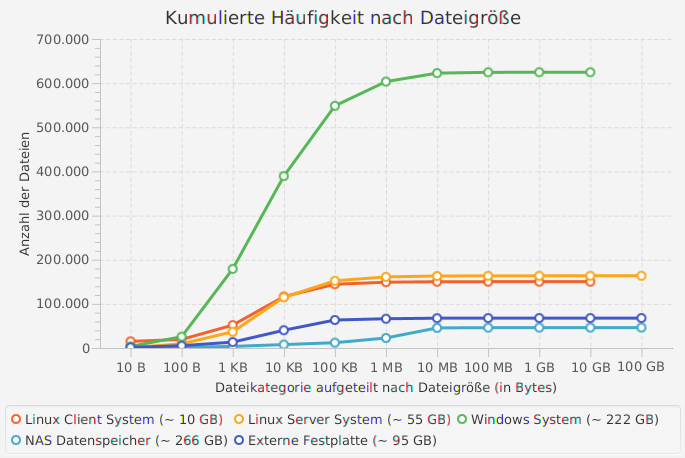
\includegraphics[width=\textwidth]{./resource/fileSize_cumulatedAmount.png}
  \caption{Kumulierte Häufigkeit nach Dateigröße}
  \label{fig:file_size_c_amount}
\end{figure}

\noindent
Nachfolgend werden die Testdaten beschrieben:
\begin{itemize}
\item Das \textit{Linux Client System} ist ungefähr 9 GB\footnote{Die Größenangaben entsprechen den reinen Rohdaten der Dateien. Verzeichnisse und Dateisystemmetadaten sind nicht inkludiert.} groß und enthält ein Ubuntu-Betriebsystem. Es wurde als Testdatenträgerabbild im Rahmen Masterthesis erstellt. Das Abbild enthält 150.229 Dateien.\footnote{Es handelt sich ausschließlich um Datendateien. Verzeichnisse, Symbolische Links und Spezielle Dateien wurden nicht berücksichtigt.}
\item Das \textit{Linux Server System} ist ungefähr 51 GB groß und enthält ein CentOS-Betriebssystem. Das System ist ein Name Node eines kleinen Hadoop-Clusters. Das Abbild enthält 163.555 Dateien.
\item Das \textit{Windows System} ist ungefähr 207 GB groß und ist ein reales Nutzersystem, welches seit mehreren Monaten eingesetzt wird. Das Abbild enthält 624.650 Dateien.
\item Der \textit{NAS Datenspeicher} entspricht einem QNAP-System mit ungefähr 257 GB an realen Rohdaten. Hierbei ist auf dem Datenträgerabbild kein Betriebssystem installiert. Es handelt sich hauptsächlich um Dokumente und Mediendateien. Das Abbild enthält 46.215 Dateien.
\item Die \textit{Externe Festplatte} mit ungefähre 90 GB Daten, wird als Backup für diverse Mediendateien genutzt. Das Abbild enthält 67.809 Dateien.
\end{itemize}

\noindent
Da die forensische Analyseplattform mehrere Datenträgerabbilder speichern kann, sollte das System durchaus mehrere Millionen Dateien verarbeiten können. Abbildung \ref{fig:file_size_r_c_amount} relativiert die Ergebnisse der einzelnen Abbilder.\\

 \begin{figure}[ht]
  \centering
  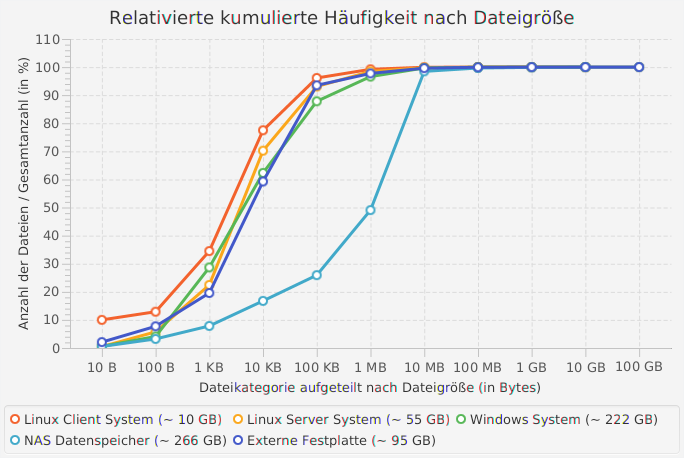
\includegraphics[width=\textwidth]{./resource/fileSize_relativeCumulatedAmount.png}
  \caption{Relativierte kumulierte Häufigkeit nach Dateigröße}
  \label{fig:file_size_r_c_amount}
\end{figure}

\noindent
Anhand der relativierten kumulativen Häufigkeit aus Abbildung \ref{fig:file_size_r_c_amount} wird klar, dass fast 80-90 \% der Dateien kleiner 100 Kilobyte sind und mehr als 95\% der Dateien kleiner 10 Megabyte sind. Allerdings sind diese Angaben mit Vorsicht zu genießen, denn je nach Anwendungsfall können Datenträger beliebige Dateien unterschiedlicher Größe speichern. Ist beispielsweise ein Betriebssystem auf dem Datenträger installiert, existieren allein durch das Betriebssystem tausende von Dateien mit minimaler Dateigröße. Umgekehrt enthält das Datenträgerabbild des NAS-Datenspeichers sehr viele Dateien zwischen 1 und 10 MB. Dies liegt daran, dass von den 46.215 Dateien ungefähr 30.000 Dateien Fotos sind. Diese wiederum sind für gewöhnlich 500 Kilobyte bis 10 Megabyte groß. Die Kurve könnte allerdings anders aussehen, wenn beispielsweise auch Filme und Videos auf dem NAS gespeichert wären.\\

\noindent
Die nachfolgende Abbildung \ref{fig:file_size_c_file_size} und die Abbildung \ref{fig:file_size_r_c_file_size} zeigen die absolute und relativierte kumulative Kategoriegröße der einzelnen Kategorien an. Die Kategoriegröße beschreibt die Gesamtgröße aller Dateien einer spezifischen Kategorie. Beispielsweise sind bei dem Windows System ungefähr 80 Gigabyte der Gesamtdatengröße in Dateien kleiner 10 Megabyte gespeichert.\\  

 \begin{figure}[ht]
  \centering
  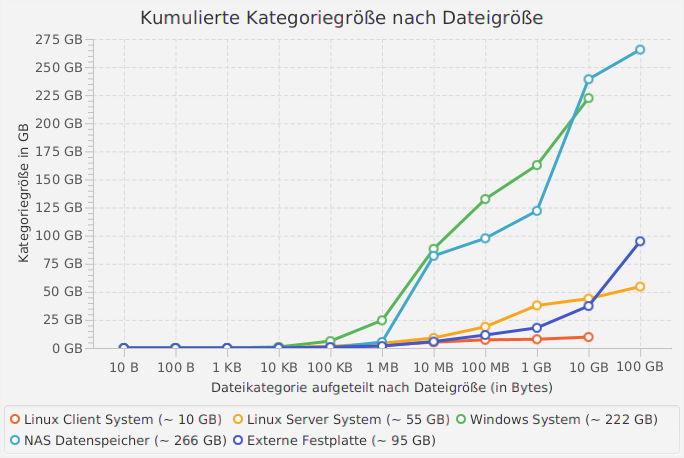
\includegraphics[width=\textwidth]{./resource/fileSize_cumulatedCategorieSize.png}
  \caption{Kumulierte Kategoriegröße nach Dateigröße}
  \label{fig:file_size_c_file_size}
\end{figure}

\noindent
Die relativierte kumulative Kategoriegröße in Abbildung \ref{fig:file_size_r_c_file_size} verdeutlicht den Kontrast in Bezug auf die relativierte kumulative Häufigkeit aus Abbildung \ref{fig:file_size_r_c_amount}. Während mehr als 95\% aller Dateien kleiner 10 Megabyte sind, beansprucht dieser Anteil doch nur ungefähr 10 bis 55 \% der Gesamtspeichergröße.\\

\noindent
Anhand der Diagramme empfiehlt es sich den Grenzwert der Dateigröße zwischen 1 und 10 Megabyte zu definieren. Für die Implementierung im Rahmen der Thesis wird der Grenzwert für die forensische Analyseplattform auf 10 Megabyte gesetzt. Dies bedeutet, dass alle Dateien kleiner 10 Megabyte direkt in HBASE gespeichert werden. Darunter fallen beispielsweise auch größtenteils Fotos und Dokumente. Und nur die wenigen großen Dateien (größer 10 Megabyte) werden direkt im HDFS gespeichert.  

 \begin{figure}[ht]
  \centering
  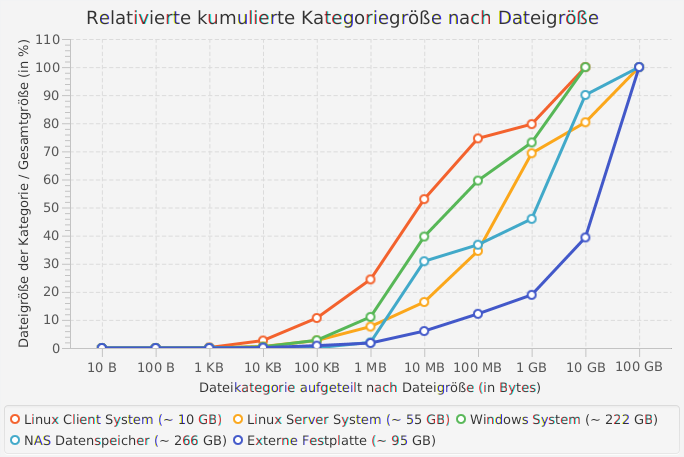
\includegraphics[width=\textwidth]{./resource/fileSize_relativeCumulatedCategorieSize.png}
  \caption{Relativierte kumulierte Kategoriegröße nach Dateigröße}
  \label{fig:file_size_r_c_file_size}
\end{figure}

\subsubsection{Aufbau der Anwendung} 
 
Diese Variante beschreibt einen Ansatz, bei welchem die Metadaten und sehr kleine Dateien direkt in HBASE persistiert werden. Dateien ab einer bestimmten Größe (derzeit ab 10 MB Dateigröße) werden direkt im HDFS abgelegt und im jeweiligen Dateieintrag in HBASE verlinkt. Auch hier muss beim Import der Daten eine eigene Anwendung die Informationen aus dem Datenträgerabbild auslesen und entsprechend ihrer Struktur in HBASE und HDFS speichern. Das GitHub-Projekt \textit{foam-data-import} enthält diese Anwendung (siehe \url{https://github.com/jobusam/foam-data-import}).\\
Abbildung \ref{fig:data_import} skizziert die Datenaufbereitung und Speicherung in HBASE und im HDFS.\\
\begin{figure}[ht]
  \centering
  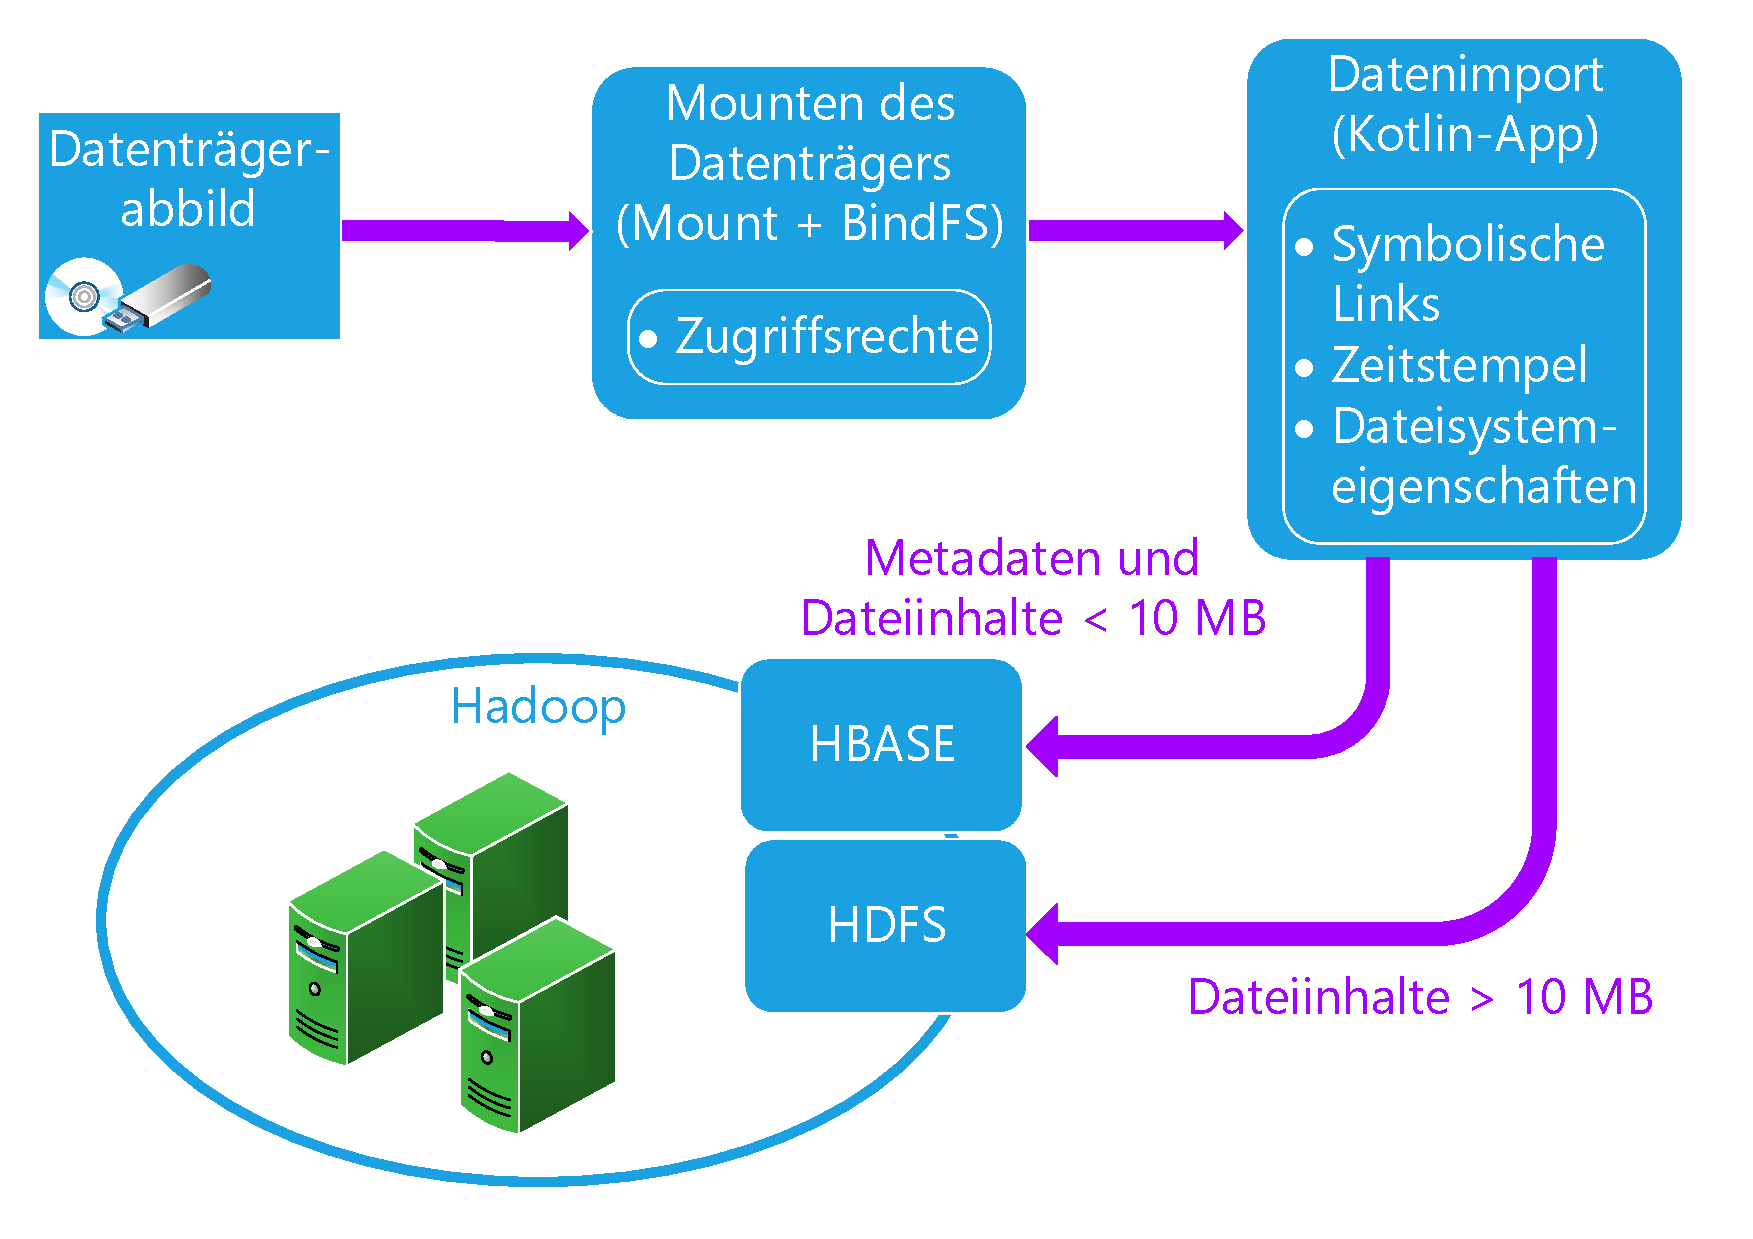
\includegraphics[width=\textwidth]{./resource/storage_hdfs_and_hbase.pdf}
  \caption{Datenimport in HBASE und HDFS}
  \label{fig:data_import}
\end{figure}

\noindent


\subsubsection{Datenmodell}

Das Datenmodell beschreibt die Struktur der Metadaten und verdeutlicht den Informationsgehalt der forensischen Analyseplattform. 

\begin{table}[!ht]
\centering
\begin{tabular}{|l|l|p{8cm}|}\hline
\bfseries Spaltenfamilie & \bfseries Spaltenname & \bfseries Beschreibung
\csvreader[head to column names]{resource/hbase_datamodel.csv}{}
{\\\hline \columnfamily & \column & \description}\\\hline
\end{tabular}
\caption{Datenmodell in HBASE}
\label{tab:hbase_datamodel}
\end{table}

TODO: Datenimport mit unterschiedlicher Dateigröße aufzeigen.
Dies zeigt sich auch bei den Testdaten. Auf einem 10 GB großen Testdatenträgerabbild wurde ein Ubuntu-Linux installiert und einige Nutzeroperationen durchgeführt. Nachfolgende Abbildung zeigt die Anzahl der Dateien gruppiert nach deren Größe. Hier wird deutlich, dass es bei der Analyse von Datenträgern primär um das Verarbeiten sehr vieler und sehr kleiner Dateien geht. \\

\noindent
Ein weitere Punkt ist auch die technische Speicherung. In einem einzelnen HDFS-Verzeichnis können maximal 32000 Dateien gespeichert werden?! Hingegen können in einem lokalen Verzeichnis eines ext4-Dateisystems deutlich mehr Dateien gespeichert werden. Bei einem Datenträgerabbild welches mehr als 1048576\footnote{Siehe Konfiguration von \textit{dfs.namenode.fs-limits.max-directory-items}. Dieser Wert kann maximal auf 6.400.000 gesetzt werden. Siehe \url{https://hadoop.apache.org/docs/r3.0.0/hadoop-project-dist/hadoop-hdfs/hdfs-default.xml} Stand: 23.8.2018.} Dateien in einem Verzeichnis speichert, müsst im HDFS ein zweites Verzeichnis zur Speicherung angelegt werden. Somit ist es auch technisch nicht möglich die gleiche logische Verzeichnisstruktur im HDFS aufzubauen. Mit dieser Variante können bei Bedarf wenigstens neue Verzeichnisse im HDFS angelegt werden!
Bei dem Windows-Verzeichnis sind bereits 2000 Dateien größer 10 MB.


%\noindent
%TODO: Siehe HBASE MOB (Medium-sized Object Binaries)
TODO: Fazit der vor und nachteile aller varianten, um zu zeigen wie variante 2 besser als 1 ist und variante 3 besser als 2 wäre und variante 4 die beste variante ist!
\section{Fachliche Probleme bei den Daten}

\subsection{Symbolische Links}
Es gibt einige Hürden beim Importieren der Datenträger in das HDFS. Wie bereits erwähnt werden die Daten auf logischer Dateiebene in das Hadoop-System importiert. Hierbei müssen spezielle Dateitypen berücksichtigt werden. Ein Beispiel ist die Verarbeitung von symbolischen Links, welche gerade unter Linux-basierten Betriebssystemen beziehungsweise in der EXT-Dateisystemfamilie auftreten können. Denn wenn symbolische Links in einem Dateisystem gespeichert werden und letzteres im Analysesystem gemountet wird, so können diese Links auch auf Dateien außerhalb des Dateisystems verweisen. Denn letztlich interpretiert das Betriebssystem diese symbolischen Links. Bei der forensischen Analyse könnte diese aber zu schwerwiegenden Fehlern der Analyseergebnisse führen, wenn beispielsweise Inhalte des Analyserechners verarbeitet werden, welche ursprünglich nicht auf dem Asservat vorhanden waren. Daher muss beim Import auf geprüft werden, ob die Datei einem symbolischen Link entspricht. Ist dies der Fall darf, der symbolische Link nicht interpretiert werden. 

\subsection{Zugriffsrechte}
Ein weiterer Aspekt ist die Beschränkung der Dateizugriffe auf Basis der vorgegebenen Zugriffsrechte. Angenommen es wird ein Datenträgerabbild auf einem Analysesystem gemountet.
Dann kann dies im Normalfall nur mit Root-Rechten durchgeführt werden. 
Der forensische Analyse benötigt also zumindest auf seinem Analyse-Rechner 
privilegierte Ausführungsrechte.\\
Beim Import von Dateien auf eben diesem gemounteten Dateisystem des Datenträgerabbildes sind jedoch die Dateizugriffsrechte weitaus interessanter. Denn das Analyse-Betriebssystem berücksichtigt diese Zugriffsrechte. Während diese Problematik beispielsweise bei NTFS-Dateisystemen eine untergeordnete Rolle spielt, so werden hingegen bei EXT-Dateisystemen die Unix-Dateirechte gespeichert und auch auf dem Analysesystem interpretiert. 
Daher kann der Nutzer und dessen ausgeführte Programme, welche die Daten aus dem Dateisystem auslesen, nicht in allen Fällen auf alle Dateien zugreifen.\\

\noindent
Die einfachste Möglichkeit um die Problematik der Zugriffsrechte zu umgehen, wäre das Ausführen der Datenimport-Applikation mit Root-Rechten. Andererseits sollte die Datenimport-Applikation aber nicht mit Root-Rechten ausgestattet werden, da dies zu Sicherheitslücken und unvorhergesehenen Rechteausweitungen im Fehlerfall führen könnte. Darüber hinaus kann bei einem Fehlverhalten der Anwendung das Analysesystem beschädigt werden. \\
Letztlich braucht die Anwendung zum Datenimport nur die Berechtigungen zum Lesen von Dateien mit Root-Rechten. Dies würde dem \textit{Need-to-know-Prinzip} genügen.\\
%(TODO: verweis auf s. 42 M106)

\noindent
Eigentlich müsste beim Mounten des Dateisystems dem Betriebssystem mitgeteilt werden können, dass die Dateirechte des gemounteten Dateisystems ignoriert werden sollen. Diese Option ist aber nicht möglich\footnote{Zumindest konnte keine funktionierende Variante gefunden werden (siehe Man-Page des Mount-Befehls.}.\\
Eine weitere Alternative wäre die Möglichkeit mit Access Control Lists (ACL) zu arbeiten und dem nichtprivilegiertem Nutzer Rechte zum Lesen der Dateien zu geben. Oder umgekehrt alle Dateien dem nichtprivilegierten Nutzer zuzordnen, welcher wiederum den Datenimport startet.
Hierzu müsste die Datenträgerkopie schreibend gemountet werden, damit die Rechte jeder Datei angepasst werden können. Dies würde wiederum dazu führen, dass das Datenträgerabbild als sichergestelltes Asservat geändert werden würde. 
Daher ist diese Lösung auch nicht geeignet.\\

\noindent
Eine weitere Alternative ist die Nutzung von Posix Capabilities\footnote{Siehe Manpages mit folgendem Befehl: \textit{ man 7 capabilities}.}.
Dies scheint unter CentOS/Fedora wohl die beste Variante zu sein. Zum Lesenden Zugriff auf Dateien müsste die Posix Capability \textit{CAP\_DAC\_READ\_SEARCH} gesetzt werden.\\
Mit nachfolgenden Kommando könnte diese Capability dem Analyseprogramm gesetzt werden.
Damit könnte dann auch ein nicht-privilegierte Nutzer lesenden Zugriff auf privilegierte Dateien erhalten.\\ 

\begin{lstlisting}[label={lst:pos_cap_command},caption= Befehl zum Setzen von Posix Capabilities,captionpos=b,frame=single,style=customshell]
setcap CAP_DAC_READ_SEARCH /bin/forensic_import
\end{lstlisting}
% Mit oder ohne + eip???
%setcap CAP\_DAC\_READ\_SEARCH+eip /bin/ping

\noindent
Allerdings funktioniert diese Art hauptsächlich bei Binärprogrammen aber nicht bei Shell-Skripten oder Java-Anwendungen. Ein ähnliche Alternative zu Posix Capabilities ist das Setzen des SUID-Bits als Unix-Dateirecht für die Programmdatei. Aber auch gilt wieder, dass dies für Binärprogramme funktioniert aber nicht für interpretierte Skripte oder Java-Anwendungen, welche wiederum in der Java Virtual Machine laufen.
%Setzen des Flags
%chmod u-s /bin/ping

Die Nutzung von SELINUX empfiehlt sich hier auch nicht. SELINUX ist eine Erweiterung des Linux-Kernels um detaillierte Zugriffskontrollen zu setzen. Diese Erweiterung ermöglicht eine detaillierte Definition, welche Anwendung oder Nutzer auf einzelne Dateien zugreifen dürfen. Allerdings werden auch unter SELINUX immer zuerst die Unix-Dateirechte und zusätzlich die in SELINUX definierten Zugriffskontrollen geprüft. Daher kann auch mit SELINUX das Problem nicht behoben werden.\\

\noindent
Zuletzt gibt es noch eine Variante, welche die Problematik mit den Dateirechten lösen kann. 
Mit dem Projekt \textit{bindfs}\footnote{Siehe \url{https://bindfs.org/}.} können unter Linux Dateisystemverzeichnisse neu gemountet werden und ihre Zugriffsrechte verändert werden. Der nachfolgende Befehl mountet das existierende Verzeichnis mit den enthaltenden Dateien in einem neuen Verzeichnis und setzt beispielsweise bei jeder Datei die aktuelle ID des Nutzers als Datei-Owner und Group. 
\begin{lstlisting}[label={lst:bindfs_command},caption= Nutzung von Bindfs zum Ändern von Dateirechten,captionpos=b,frame=single,style=customshell]
sudo bindfs -u $(id -u) -g $(id -g) src_dir/ target_dir/
\end{lstlisting}
Der Befehl selbst benötigt Root-Rechte. Jedoch kann der Nutzer danach alle Dateien des Zielverzeichnisses lesen. Der einzige Nachteil an dieser Lösung ist, dass der Besitzer und die Gruppe jeder einzelnen Datei nun der Nutzer des Analysesystems ist.\\
Dieser Nachteil muss zukünftig behoben werden, damit die forensische Analyseplattform auch die Besitzer und Gruppen einer Datei korrekt auswerten kann.
%Im Anhang beschreiben, wie bindfs gebaut werden kann.